%%%%%%%%%%%%%%%%%%%%%%%%%%%%%%%%%%%%%%%%%%%%%%%%%%%%%%%%%%%%%%%%%%%%%%%%
%% Customizações do abnTeX2 (http://abnTeX2.googlecode.com)           %%
%% para a Universidade de Fortaleza						              %%
%%                                                                    %%
%% This work may be distributed and/or modified under the             %%
%% conditions of the LaTeX Project Public License, either version 1.3 %%
%% of this license or (at your option) any later version.             %%
%% The latest version of this license is in                           %%
%%   http://www.latex-project.org/lppl.txt                            %%
%% and version 1.3 or later is part of all distributions of LaTeX     %%
%% version 2005/12/01 or later.                                       %%
%%                                                                    %%
%% This work has the LPPL maintenance status `maintained'.            %%
%%                                                                    %%
%% The Current Maintainer of this work is Bruno Lopes                 %%
%%                                                                    %%
%% Project available on: https://github.com/david-fbuni/fbunitex2   %%
%%                                                                    %%
%% Further information about abnTeX2                                  %%
%% are available on http://abntex2.googlecode.com/                    %%
%%                                                                    %%
%%%%%%%%%%%%%%%%%%%%%%%%%%%%%%%%%%%%%%%%%%%%%%%%%%%%%%%%%%%%%%%%%%%%%%%%

\documentclass[
    a4paper,          % Tamanho da folha A4
    12pt,             % Tamanho da fonte 12pt
    chapter=TITLE,    % Todos os capitulos devem ter caixa alta
    section=TITLE,    % Todas as secoes devem ter caixa alta
    oneside,          % Usada para impressao em apenas uma face do papel
    english,          % Hifenizacoes em ingles
    spanish,          % Hifenizacoes em espanhol
    brazil            % Ultimo idioma eh o idioma padrao do documento
]{abntex2}

% Importações de pacotes
\usepackage[brazil]{babel} 
\usepackage[utf8]{inputenc}                         % Acentuação direta
\usepackage[T1]{fontenc}                            % Codificação da fonte em 8 bits
\usepackage{graphicx}                               % Inserir figuras
\usepackage{amsfonts, amssymb, amsmath}             % Fonte e símbolos matemáticos
\usepackage{booktabs}                               % Comandos para tabelas
\usepackage{verbatim}                               % Texto é interpretado como escrito no documento
\usepackage{multirow, array}                        % Múltiplas linhas e colunas em tabelas
\usepackage{indentfirst}                            % Endenta o primeiro parágrafo de cada seção.
\usepackage{listings}                               % Utilizar codigo fonte no documento
\usepackage{xcolor}
\usepackage{microtype}                              % Para melhorias de justificação?
\usepackage[portuguese,ruled,lined]{algorithm2e}    % Escrever algoritmos
\usepackage{algorithmic}                            % Criar Algoritmos
%\usepackage{float}                                  % Utilizado para criação de floats
\usepackage{amsgen}
\usepackage{lipsum}                                 % Usar a simulação de texto Lorem Ipsum
%\usepackage{titlesec}                               % Permite alterar os títulos do documento
\usepackage{tocloft}                                % Permite alterar a formatação do Sumário
\usepackage{etoolbox}                               % Usado para alterar a fonte da Section no Sumário
\usepackage[nogroupskip,nonumberlist,acronym]{glossaries}                % Permite fazer o glossario
\usepackage{caption}                                % Altera o comportamento da tag caption
\usepackage[alf, abnt-emphasize=bf, bibjustif, recuo=0cm, abnt-etal-cite=3, abnt-etal-list=0,abnt-etal-text=it]{abntex2cite}  % Citações padrão ABNT
%\usepackage[bottom]{footmisc}                      % Mantém as notas de rodapé sempre na mesma posição
%\usepackage{times}                                 % Usa a fonte Times
\usepackage{mathptmx}                               % Usa a fonte Times New Roman
\usepackage{lmodern}                               % Usa a fonte Latin Modern
%\usepackage{subfig}                                % Posicionamento de figuras
%\usepackage{scalefnt}                              % Permite redimensionar tamanho da fonte
%\usepackage{color, colortbl}                       % Comandos de cores
%\usepackage{lscape}                                % Permite páginas em modo "paisagem"
%\usepackage{ae, aecompl}                           % Fontes de alta qualidade
%\usepackage{picinpar}                              % Dispor imagens em parágrafos
%\usepackage{latexsym}                              % Símbolos matemáticos
%\usepackage{upgreek}                               % Fonte letras gregas
\usepackage{appendix}                               % Gerar o apendice no final do documento
\usepackage{paracol}                                % Criar paragrafos sem identacao
\usepackage{lib/fbunitex2}		                    % Biblioteca com as normas da fbuni para trabalhos academicos
\usepackage{pdfpages}                               % Incluir pdf no documento
\usepackage{amsmath}                                % Usar equacoes matematicas
\usepackage{Environ}
\usepackage{cooltooltips}


% Estas linhas referência a 
\usepackage{catchfilebetweentags}
\newcommand{\loadFigure}[1]{ % define command to load figures
	\ExecuteMetaData[figures.tex]{#1} % call the package macro to load chunk from file
}

\newcommand{\loadPergunta}[1]{ % define command to load figures
	\ExecuteMetaData[perguntas.tex]{#1} % call the package macro to load chunk from file
}


% Update filecontents* environment to overwrite by default
\expandafter\let\expandafter\filecontentsstar\csname filecontents*\endcsname
\expandafter\let\expandafter\endfilecontentsstar\csname endfilecontents*\endcsname
\RenewEnviron{filecontents*}[2][overwrite]{%
	\begin{filecontentsstar}[#1]{#2}
		\BODY
	\end{filecontentsstar}
}


% Estas linhas referência aos Pie chart
\RequirePackage{tikz}
\RequirePackage{pgf-pie}

% Estas linhas referência aos Horizontal Bar chart
\usepackage{pgfplots}
\usepackage{pgfplotstable}
\pgfplotsset{compat=1.7}
%\documentclass[tikz]%{standalone}
\usepackage{bchart}
\usetikzlibrary{decorations.pathreplacing}
\definecolor{RYB2}{RGB}{245,245,245}
\definecolor{RYB1}{RGB}{218,232,252}
\definecolor{RYB4}{RGB}{108,142,191}

% Estas linhas referência ao Orgchart
\usepackage[edges]{forest}
\usetikzlibrary{arrows.meta,shapes,positioning,shadows,trees,fit}
\tikzset{
	basic/.style  = {draw, text width=2cm, drop shadow, font=\sffamily, rectangle},
	basic1/.style  = {draw,  drop shadow, font=\sffamily, rectangle},
	root/.style   = {basic, rounded corners=2pt, thin, align=center, fill=green!30},
	basic2/.style  = {draw,  drop shadow, font=\sffamily, rectangle},
	root/.style   = {basic, rounded corners=2pt, thin, align=center, fill=green!30},
	onode/.style = {basic, thin, rounded corners=2pt, align=center, fill=green!60, text width=3cm,},
	tnode/.style = {basic1, thin, align=left, fill=pink!60, text width=6.5em},
	dnode/.style = {basic2, thin, align=left, fill=yellow!60, text width=6.5em},
	edge from parent/.style={draw=black, edge from parent fork right},
	fitbox/.style = {draw, gray, dashed, inner ysep=5pt, inner xsep=7.5pt, rounded corners=2pt},
}
\forestset{
	fitting/.style={
		tikz={\node [fitbox, fit=#1] {};},
		no edge,
		inner ysep=0pt,
	}
}

% Esta linha referência garantir que as figuras apareçam na seção a que estão associadas?
\usepackage[section]{placeins}

\makeatletter
\AtBeginDocument{%
	\expandafter\renewcommand\expandafter\subsection\expandafter{%
		\expandafter\@fb@secFB\subsection
	}%
}
\makeatother

% Esta linha referência ao centralização do 1° título da tabela
\newcolumntype{P}[1]{>{\centering\arraybackslash}m{#1}}


% Organiza e gera a lista de abreviaturas, simbolos e glossario
\makeglossaries

% Gera o Indice do documento
\makeindex
%%%%%%%%%%%%%%%%%%%%%%%%%%%%%%%%%%%%%%%%%%%%%%%%%%%%%
%%          Configuracoes Personalizadas           %%
%%%%%%%%%%%%%%%%%%%%%%%%%%%%%%%%%%%%%%%%%%%%%%%%%%%%%

% Esta linha referência as numeração sequencial label.
\usepackage{chngcntr}
\counterwithin{figure}{chapter}
\counterwithin{table}{chapter}

%%%%%%%%%%%%%%%%%%%%%%%%%%%%%%%%%%%%%%%%%%%%%%%%%%%%%
%%     Final de  Configuracoes Personalizadas      %%
%%%%%%%%%%%%%%%%%%%%%%%%%%%%%%%%%%%%%%%%%%%%%%%%%%%%%
%%%%%%%%%%%%%%%%%%%%%%%%%%%%%%%%%%%%%%%%%%%%%%%%%%%%%%%%%%%%%%%%%%%%%%%%%
%% Customizações do abnTeX2 (http://abnTeX2.googlecode.com)           %%
%% para a Universidade de Fortaleza						              %%
%%                                                                    %%
%% This work may be distributed and/or modified under the             %%
%% conditions of the LaTeX Project Public License, either version 1.3 %%
%% of this license or (at your option) any later version.             %%
%% The latest version of this license is in                           %%
%%   http://www.latex-project.org/lppl.txt                            %%
%% and version 1.3 or later is part of all distributions of LaTeX     %%
%% version 2005/12/01 or later.                                       %%
%%                                                                    %%
%% This work has the LPPL maintenance status `maintained'.            %%
%%                                                                    %%
%% The Current Maintainer of this work is Bruno Lopes                 %%
%%                                                                    %%
%% Project available on: https://github.com/bruno-unifor/unifortex2   %%
%%                                                                    %%
%% Further information about abnTeX2                                  %%
%% are available on http://abntex2.googlecode.com/                    %%
%%                                                                    %%
%%%%%%%%%%%%%%%%%%%%%%%%%%%%%%%%%%%%%%%%%%%%%%%%%%%%%%%%%%%%%%%%%%%%%%%%

\documentclass[
    a4paper,          % Tamanho da folha A4
    12pt,             % Tamanho da fonte 12pt
    chapter=TITLE,    % Todos os capitulos devem ter caixa alta
    section=TITLE,    % Todas as secoes devem ter caixa alta
    oneside,          % Usada para impressao em apenas uma face do papel
    english,          % Hifenizacoes em ingles
    spanish,          % Hifenizacoes em espanhol
    brazil            % Ultimo idioma eh o idioma padrao do documento
]{abntex2}

% Importações de pacotes
\usepackage[brazil]{babel} 
\usepackage[utf8]{inputenc}                         % Acentuação direta
\usepackage[T1]{fontenc}                            % Codificação da fonte em 8 bits
\usepackage{graphicx}                               % Inserir figuras
\usepackage{amsfonts, amssymb, amsmath}             % Fonte e símbolos matemáticos
\usepackage{booktabs}                               % Comandos para tabelas
\usepackage{verbatim}                               % Texto é interpretado como escrito no documento
\usepackage{multirow, array}                        % Múltiplas linhas e colunas em tabelas
\usepackage{indentfirst}                            % Endenta o primeiro parágrafo de cada seção.
\usepackage{listings}                               % Utilizar codigo fonte no documento
\usepackage{xcolor}
\usepackage{microtype}                              % Para melhorias de justificação?
\usepackage[portuguese,ruled,lined]{algorithm2e}    % Escrever algoritmos
\usepackage{algorithmic}                            % Criar Algoritmos
%\usepackage{float}                                  % Utilizado para criação de floats
\usepackage{amsgen}
\usepackage{lipsum}                                 % Usar a simulação de texto Lorem Ipsum
%\usepackage{titlesec}                               % Permite alterar os títulos do documento
\usepackage{tocloft}                                % Permite alterar a formatação do Sumário
\usepackage{etoolbox}                               % Usado para alterar a fonte da Section no Sumário
\usepackage[nogroupskip,nonumberlist,acronym]{glossaries}                % Permite fazer o glossario
\usepackage{caption}                                % Altera o comportamento da tag caption
\usepackage[alf, abnt-emphasize=bf, bibjustif, recuo=0cm, abnt-etal-cite=3, abnt-etal-list=0,abnt-etal-text=it]{abntex2cite}  % Citações padrão ABNT
%\usepackage[bottom]{footmisc}                      % Mantém as notas de rodapé sempre na mesma posição
%\usepackage{times}                                 % Usa a fonte Times
\usepackage{mathptmx}                               % Usa a fonte Times New Roman
%\usepackage{lmodern}                               % Usa a fonte Latin Modern
%\usepackage{subfig}                                % Posicionamento de figuras
%\usepackage{scalefnt}                              % Permite redimensionar tamanho da fonte
%\usepackage{color, colortbl}                       % Comandos de cores
%\usepackage{lscape}                                % Permite páginas em modo "paisagem"
%\usepackage{ae, aecompl}                           % Fontes de alta qualidade
%\usepackage{picinpar}                              % Dispor imagens em parágrafos
%\usepackage{latexsym}                              % Símbolos matemáticos
%\usepackage{upgreek}                               % Fonte letras gregas
\usepackage{appendix}                               % Gerar o apendice no final do documento
\usepackage{paracol}                                % Criar paragrafos sem identacao
\usepackage{lib/unifortex2}		                    % Biblioteca com as normas da Unifor para trabalhos academicos
\usepackage{pdfpages}                               % Incluir pdf no documento
\usepackage{amsmath}                                % Usar equacoes matematicas

% Organiza e gera a lista de abreviaturas, simbolos e glossario
\makeglossaries

% Gera o Indice do documento
\makeindex

% Esta linha referência ao textos de comentários e perguntas
\NewEnviron{commentA}{}
\newcommand\Aon{\RenewEnviron{commentA}{\color{red}\BODY}}
\newcommand\Aoff{\RenewEnviron{commentA}{}}
\NewEnviron{commentB}{}
\newcommand\Bon{\RenewEnviron{commentB}{\color{blue}\BODY}}
\newcommand\Boff{\RenewEnviron{commentB}{}}
\NewEnviron{commentC}{}
\newcommand\Con{\RenewEnviron{commentC}{\color{cyan}\BODY}}
\newcommand\Coff{\RenewEnviron{commentC}{}}

%%%%%%%%%%%%%%%%%%%%%%%%%%%%%%%%%%%%%%%%%%%%%%%%%%%%%
%%          Configuracoes do fbuniTeX2            %%
%%%%%%%%%%%%%%%%%%%%%%%%%%%%%%%%%%%%%%%%%%%%%%%%%%%%%

% Opcoes disponiveis

%% Trabalho final de GRADUAÇÃO no qual a folha de aprovação será um arquivo PDF
%\trabalhoacademico{tccgraduacaoPDF}

%% Trabalho final de GRADUAÇÃO no qual a folha de aprovação será gerada pelo modelo fbuniTEX
\trabalhoacademico{tccgraduacao}

%% Trabalho final de ESPECIALIZAÇÃO no qual a folha de aprovação será gerada pelo modelo fbuniTEX
%\trabalhoacademico{tccespecializacao}

%% Trabalho final de MESTRADO no qual a folha de aprovação será gerada pelo modelo fbuniTEX
%\trabalhoacademico{dissertacao}

%% Trabalho final de DOUTORADO no qual a folha de aprovação será gerada pelo modelo fbuniTEX
%\trabalhoacademico{tese}

% Define se o trabalho eh uma qualificacao
% Coloque 'nao' para versao final do trabalho

\ehqualificacao{nao}

% Remove as bordas vermelhas e verdes do PDF gerado
% Coloque 'sim' pare remover

\removerbordasdohyperlink{sim}

% Adiciona a cor Azul a todos os hyperlinks

\cordohyperlink{nao}

%%%%%%%%%%%%%%%%%%%%%%%%%%%%%%%%%%%%%%%%%%%%%%%%%%%%%
%%          Informação sobre a IES                 %%
%%%%%%%%%%%%%%%%%%%%%%%%%%%%%%%%%%%%%%%%%%%%%%%%%%%%%

\ies{Centro Universitário Farias Brito}
\iessigla{FBUNI}
\centro{Centro de Administração}

%%%%%%%%%%%%%%%%%%%%%%%%%%%%%%%%%%%%%%%%%%%%%%%%%%%%%
%%        Informação para TCC de Graduacao         %%
%%%%%%%%%%%%%%%%%%%%%%%%%%%%%%%%%%%%%%%%%%%%%%%%%%%%%

\graduacaoem{Marketing}
\habilitacao{bacharel} % Pode colocar tambem 'licenciada'

%%%%%%%%%%%%%%%%%%%%%%%%%%%%%%%%%%%%%%%%%%%%%%%%%%%%%
%%     Informação para TCC de Especializacao       %%
%%%%%%%%%%%%%%%%%%%%%%%%%%%%%%%%%%%%%%%%%%%%%%%%%%%%%

\especializacaoem{Alfabetização de Crianças}

%%%%%%%%%%%%%%%%%%%%%%%%%%%%%%%%%%%%%%%%%%%%%%%%%%%%%
%%         Informação para Dissertacao             %%
%%%%%%%%%%%%%%%%%%%%%%%%%%%%%%%%%%%%%%%%%%%%%%%%%%%%%

\programamestrado{Programa de Pós-Graduação em Informática Aplicada}
\nomedomestrado{Mestrado Acadêmico em Ciência da Computação}
\mestreem{Ciência da Computação}
\areadeconcentracaomestrado{Ciência da Computação}

%%%%%%%%%%%%%%%%%%%%%%%%%%%%%%%%%%%%%%%%%%%%%%%%%%%%%
%%               Informação para Tese              %%
%%%%%%%%%%%%%%%%%%%%%%%%%%%%%%%%%%%%%%%%%%%%%%%%%%%%%

\programadoutorado{Programa de Pós-Graduação em Informática Aplicada}
\nomedodoutorado{Doutorado em Saúde Coletiva}
\doutorem{Saúde Coletiva}
\areadeconcentracaodoutorado{Saúde Coletiva}

%%%%%%%%%%%%%%%%%%%%%%%%%%%%%%%%%%%%%%%%%%%%%%
%%  Informação relacionadas ao trabalho     %%
%%%%%%%%%%%%%%%%%%%%%%%%%%%%%%%%%%%%%%%%%%%%%%

\autor{David Nascimento da Silva}
\titulo{Marketplace de entrega de comida}
\data{2021}
\local{Fortaleza -- Ceará}

% Exemplo: \dataaprovacao{01 de Janeiro de 2017}
\dataaprovacao{01 de Junho de 2021}

%%%%%%%%%%%%%%%%%%%%%%%%%%%%%%%%%%%%%%%%%%%%%
%%     Informação sobre o Orientador       %%
%%%%%%%%%%%%%%%%%%%%%%%%%%%%%%%%%%%%%%%%%%%%%

\orientador{Raimundo Roberto Pinho}
\orientadories{Centro Universitário Farias Brito - FBUNI}
\orientadorcentro{Centro de Administração}
\orientadorfeminino{nao} % Coloque 'sim' se for do sexo feminino

%%%%%%%%%%%%%%%%%%%%%%%%%%%%%%%%%%%%%%%%%%%%%
%%      Informação sobre o Co-orientador   %%
%%%%%%%%%%%%%%%%%%%%%%%%%%%%%%%%%%%%%%%%%%%%%

% Deixe o nome do coorientador em branco para remover do documento

\coorientador{}
\coorientadories{Universidade Co-orientador - SIGLA}
\coorientadorcentro{Centro do Co-orientador - SIGLA}
\coorientadorfeminino{nao} % Coloque 'sim' se for do sexo feminino

%%%%%%%%%%%%%%%%%%%%%%%%%%%%%%%%%%%%%%%%%%%%%
%%      Informação sobre a banca           %%
%%%%%%%%%%%%%%%%%%%%%%%%%%%%%%%%%%%%%%%%%%%%%

% Atenção! Deixe o nome do membro da banca para remover da folha de aprovacao

% Exemplo de uso:
% \membrodabancadois{Prof. Dr. Fulano de Tal}
% \membrodabancadoisies{Universidade Estadual do Ceará - UECE}

\membrodabancadois{Membro da Banca Dois}
\membrodabancadoiscentro{Centro de Ciências e Tecnologia - CCT}
\membrodabancadoisies{Universidade do Membro da Banca Dois - SIGLA}

\membrodabancatres{Membro da Banca Três}
\membrodabancatrescentro{Centro de Ciências e Tecnologia - CCT}
\membrodabancatresies{Universidade do Membro da Banca Três - SIGLA}

\membrodabancaquatro{Membro da Banca Quatro}
\membrodabancaquatrocentro{Centro de Ciências e Tecnologia - CCT}
\membrodabancaquatroies{Universidade do Membro da Banca Quatro - SIGLA}

\membrodabancacinco{Membro da Banca Cinco}
\membrodabancacincocentro{Centro de Ciências e Tecnologia - CCT}
\membrodabancacincoies{Universidade do Membro da Banca Cinco - SIGLA}

\membrodabancaseis{Membro da Banca Seis}
\membrodabancaseiscentro{Centro de Ciências e Tecnologia - CCT}
\membrodabancaseisies{Universidade do Membro da Banca Seis - SIGLA}

% Esta linha referência ao textos de comentários e perguntas
\NewEnviron{commentA}{}
\newcommand\Aon{\RenewEnviron{commentA}{\color{red}\BODY}}
\newcommand\Aoff{\RenewEnviron{commentA}{}}
\NewEnviron{commentB}{}
\newcommand\Bon{\RenewEnviron{commentB}{\color{blue}\BODY}}
\newcommand\Boff{\RenewEnviron{commentB}{}}
\NewEnviron{commentC}{}
\newcommand\Con{\RenewEnviron{commentC}{\color{cyan}\BODY}}
\newcommand\Coff{\RenewEnviron{commentC}{}}


\begin{document}
	
	\Aon
	\Bon
	\Con

	% Elementos pré-textuais
	\imprimircapa
	\imprimirfolhaderosto{}
	%\imprimirfichacatalografica{elementos-pre-textuais/ficha-catalografica}
	%\imprimirerrata{elementos-pre-textuais/errata}

	%%%%%%%%%%%%%%%%%%%%%%%%%%%%%%%%%%%%%%%%%%%%%%%%%%%%%%%%%%%%%%%%%%%%%%%%%%%%%%%%%%%%%%%%%%%%%%%%%%
	%%																                               	%%
	%%		Após a defesa do TCC, a banca examinadora irá preencher a folha de aprovação,			%%
	%%		que deverá ser assinada por todos os membros da banca avaliadora e, posteriormente,		%%
	%%		deverá ser anexada na versão final do TCC pelo ALUNO.									%%
	%%																								%%
	%%		Quando tiver em mãos a folha de aprovação:												%%
	%%			1 - Escanei-a e gere um arquivo PDF													%%
	%%			2 - Renomeie o arquivo PDF para "folha-aprovacao.pdf"								%%
	%%			3 - Mova o arquivo para o diretório "elementos-pre-textuais" do modelo				%%
	%%			5 - Descomente a linha 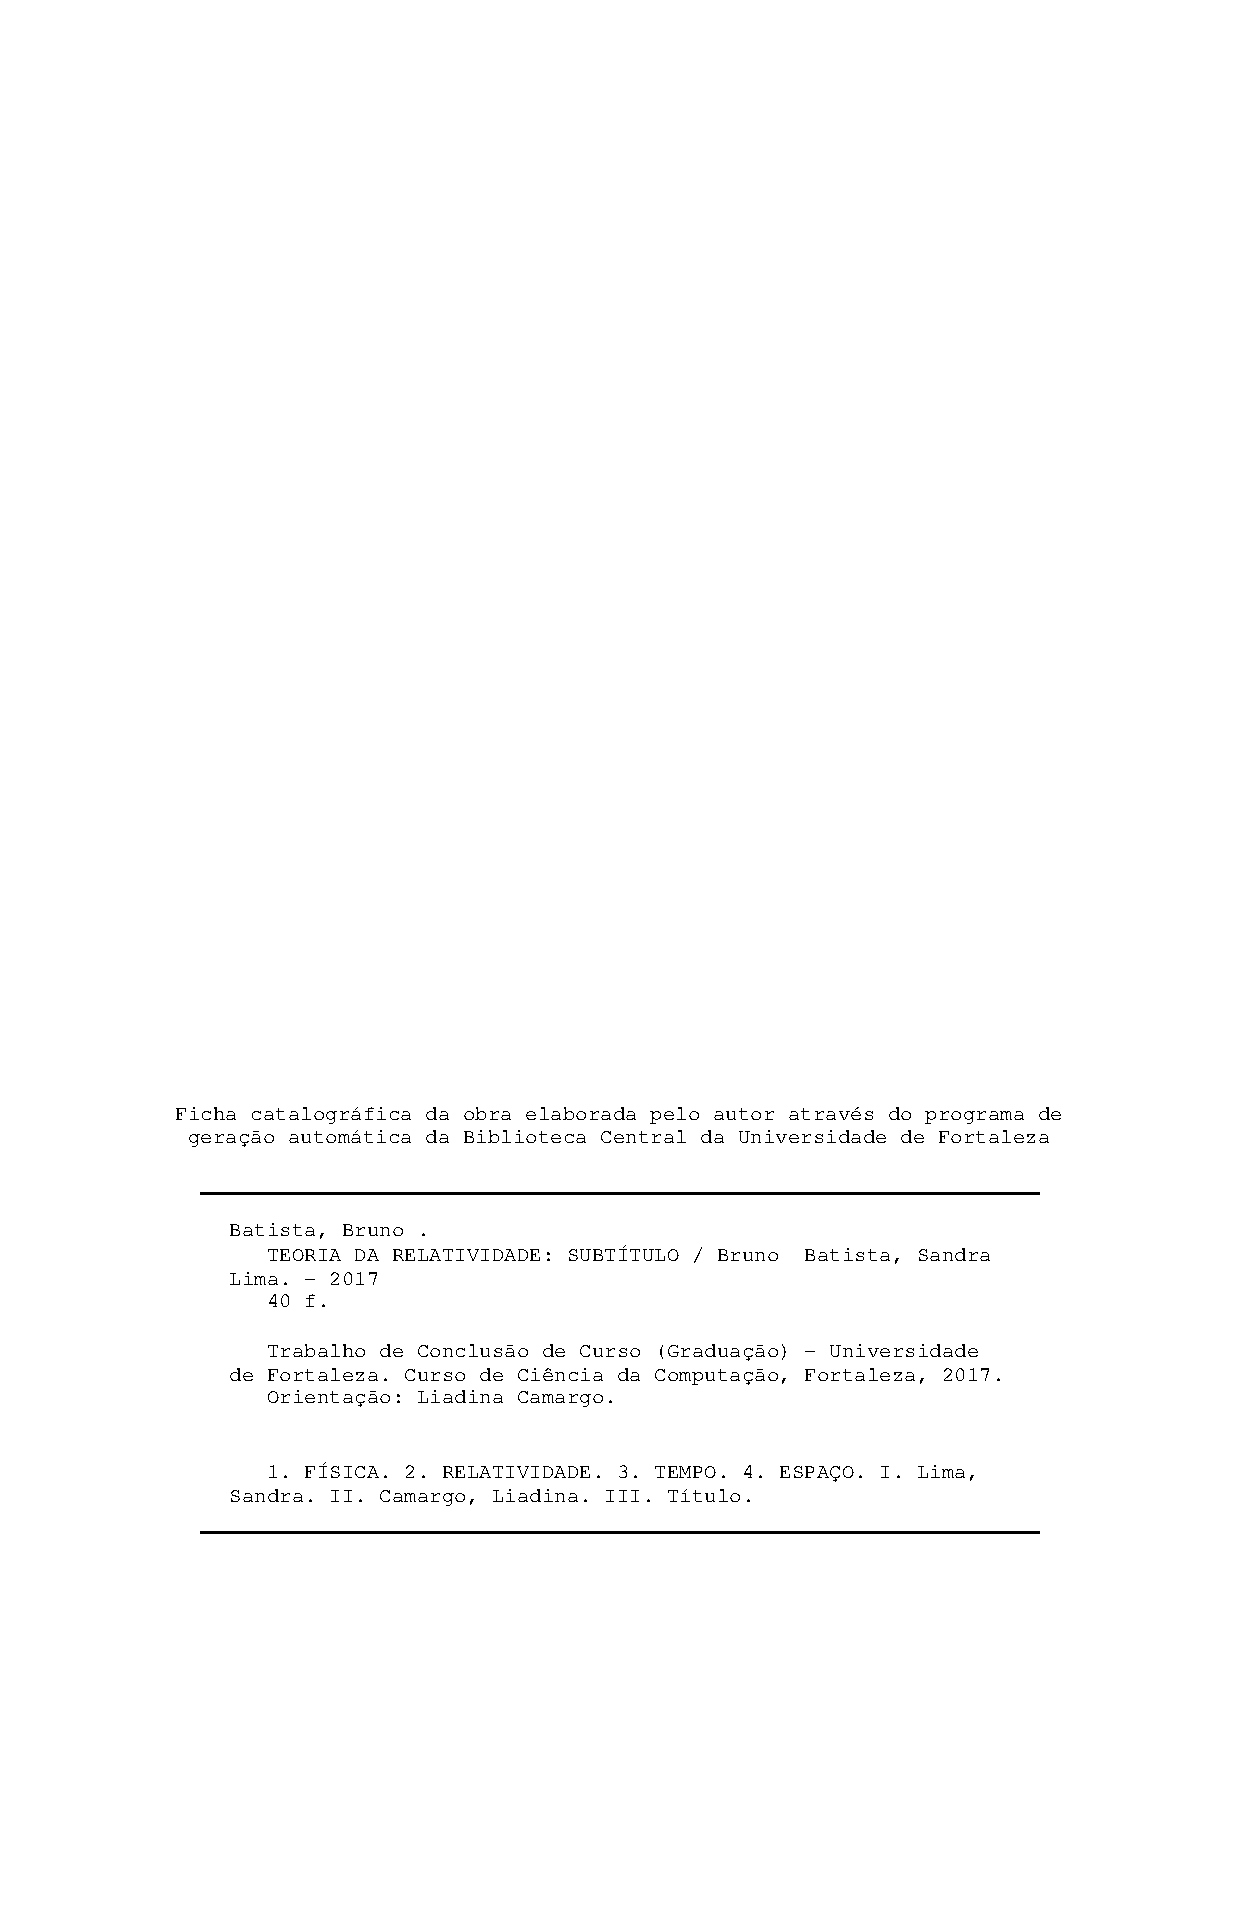
\includepdf{elementos-pre-textuais/folha-aprovacao.pdf} 		%%
	%%					removendo o simbolo de %													%%
	%%			6 - Adicione o simbolo % na linha 	\imprimirfolhadeaprovacao						%%
	%%			7 - Recompile o projeto																%%
	%%																								%%	%%%%%%%%%%%%%%%%%%%%%%%%%%%%%%%%%%%%%%%%%%%%%%%%%%%%%%%%%%%%%%%%%%%%%%%%%%%%%%%%%%%%%%%%%%%%%%%%%%
	
	%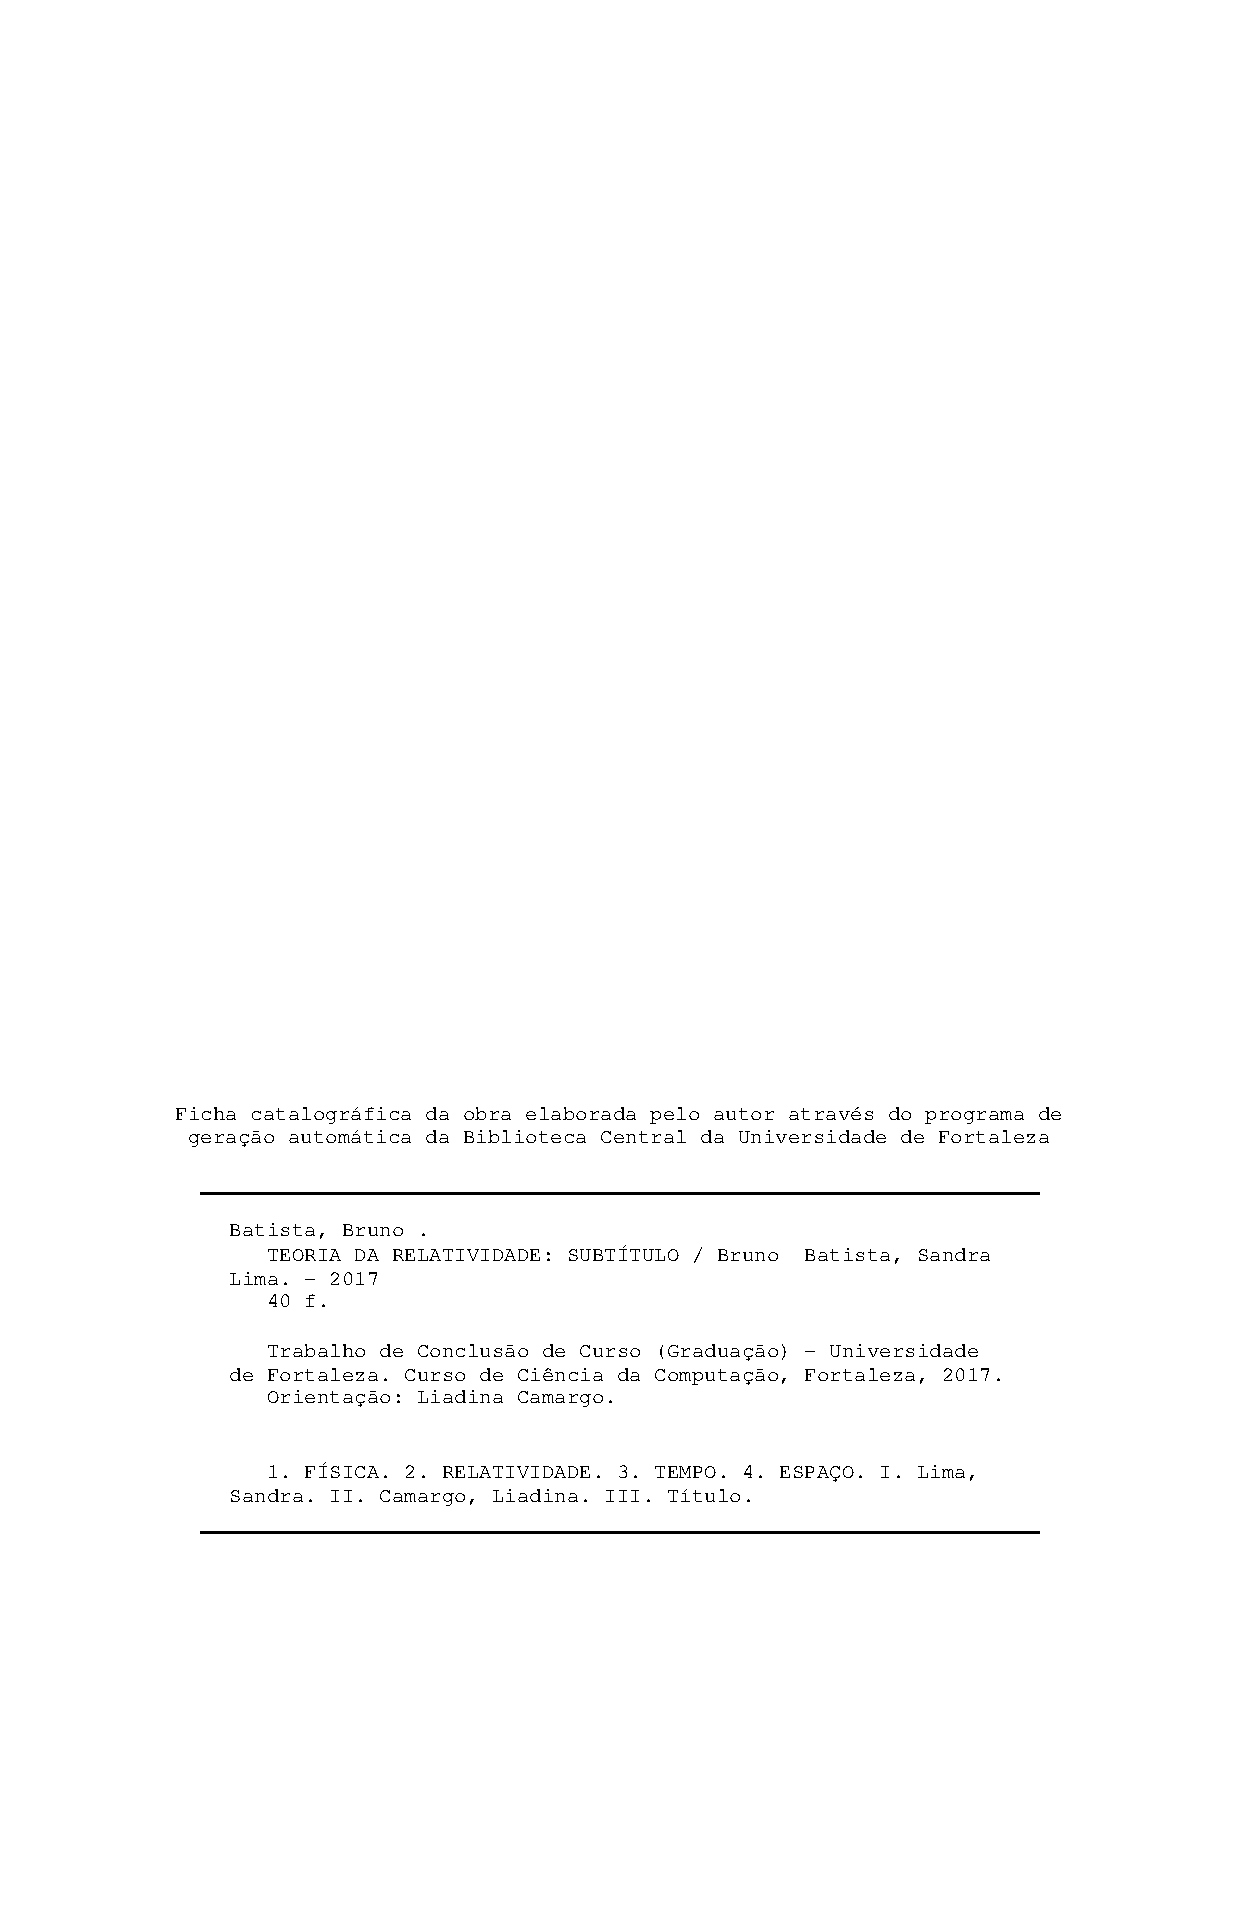
\includepdf{elementos-pre-textuais/folha-aprovacao.pdf}
	\imprimirfolhadeaprovacao
	
	%\imprimirdedicatoria{elementos-pre-textuais/dedicatoria}
	\imprimiragradecimentos{elementos-pre-textuais/agradecimentos}
	\imprimirepigrafe{elementos-pre-textuais/epigrafe}
	\imprimirresumo{elementos-pre-textuais/resumo}
	\imprimirabstract{elementos-pre-textuais/abstract}
	\imprimirlistadeilustracoes
	\imprimirlistadetabelas
	\imprimirlistadequadros
	\imprimirlistadealgoritmos
	\imprimirlistadecodigosfonte
	\imprimirlistadeabreviaturasesiglas
	\imprimirlistadesimbolos{elementos-pre-textuais/lista-de-simbolos}
	\imprimirsumario

	%Elementos textuais
	\textual
	\chapter{Introdução}
\label{cap:introducao}

\lipsum[5]
\lipsum[6]
\lipsum[7]

\section{Motivação}
\label{sec:motivacao}

\lipsum[3]
\lipsum[4]

\section{Objetivos}
\label{sec:objetivos}

Interdum et malesuada fames ac ante ipsum primis in faucibus. Lorem ipsum dolor sit amet, consectetur adipiscing elit. Ut ex tellus, sodales in euismod at, ultricies quis leo.

\subsection{Objetivo Geral}
\label{sec:objetivo-geral}

Integer imperdiet ac magna eu pulvinar. Aliquam erat volutpat. Etiam molestie, nulla a egestas aliquet, velit augue congue metus, et ultricies metus massa vel nibh. Vivamus viverra commodo finibus. Nam elementum convallis accumsan. Quisque tincidunt purus nisl, tincidunt ultricies odio ultrices eu.

\subsection{Objetivos Específicos}
\label{sec:objetivos-especificos}

Lorem ipsum dolor sit amet, consectetur adipiscing elit. Duis scelerisque, velit at facilisis hendrerit, dui eros lacinia metus, non maximus mi tortor ut lectus. Donec hendrerit leo ut consectetur tincidunt. 

	\begin{alineas}
		\item Lorem ipsum dolor sit amet, consectetur adipiscing elit. Nunc dictum sed tortor nec viverra.
		\item Praesent vitae nulla varius, pulvinar quam at, dapibus nisi. Aenean in commodo tellus. Mauris molestie est sed justo malesuada, quis feugiat tellus venenatis.
		\item Praesent quis erat eleifend, lacinia turpis in, tristique tellus. Nunc dictum sed tortor nec viverra.
		\item Mauris facilisis odio eu ornare tempor. Nunc dictum sed tortor nec viverra.
		\item Curabitur convallis odio at eros consequat pretium.
	\end{alineas}
	\chapter{Sumário Executivo}
\label{chapter:sumario}

\begin{commentA}
	
\par \end{commentA}


Neste capitulo apresenta-se uma classificação 

	
\begin{commentA}

\par \end{commentA}

\chapter{Conceito de Negócio}
\label{chapter:Conceito}


\begin{commentA} \vspace{0.3cm} \noindent Deve conter pequeno histórico da ideia.\par \vspace{0.1cm} \end{commentA}


Com 5 anos de experiência em uma grande empresa que desenvolve e licencia programas de computador customizáveis e atua em operações de mobilidade e marketplace de delivery, tenho o entendimento de melhorias de processos, para momento na área de operações em que os produtos são entregues sem danos, e as perdas causadas por mudanças ou reclamações dos clientes sobre os produtos entregues reduzida.\par

A maioria das pessoas procura um aplicativo que possa ajudá-lo a comprar comida de forma conveniente e entregar mercadorias onde quer que eu esteja sem um endereço físico, e que tenha uma interface intuitiva e fácil de usar, disponível para usar os recursos atuais processados pelo próprio aplicativo nos sistemas de smartphone mais comuns, e usar informações pessoais de forma seguras durante o registro, este é um dos principais problemas relacionados à segurança da informação.\par

Há dúvidas sobre o local a encontrar e o grau de proximidade com os usuários nos aplicativos por parte dos entregadores, que reduz a consciência dos usuários onde permanece, sobre a diversidade de opções de alimentos e produtos, o mesmo local de um produto é comum em outras categorias de alimentos, o que é outro problema.O prazo de entrega, que é um dos principais interesses dos usuários no aplicativo, desenvolver funções para que o usuário possa agendar o horário para receber o pedido sem demora.\par

O modelo de negócios da T'Entregas é uma espécie de plataforma multilateral que conecta consumidores que desejam receber alimentação com restaurantes que fornecem essa alimentação.\par


\section{\textbf{Segmento de clientes}}
\label{sec: Segmento de clientes}


\begin{commentA} \vspace{0.3cm} \noindent Quem possui o problema a ser solucionado? \par \vspace{0.1cm} \end{commentA}


Conecta consumidores que desejam receber comida delivery e restaurantes que oferecem essa modalidade de entrega. Desta forma, através do T'Entregas você pode pedir comida de diferentes restaurantes com base em seus cardápios, preços, avaliações de outros clientes e tempo de entrega estimado. O T'Entregas trata-se de um aplicativo para smartphone que oferece um marketplace com centenas de restaurantes que trabalham com entrega de comida. A oferta do aplicativo é para pessoas maiores de 18 anos, que buscam comodidade e segurança nos momentos diversos e que desejam recebe uma refeição rápida, no local que se encontrar ou onde quiser.\par


\begin{commentA} \vspace{0.3cm} \noindent Para quem criamos valor? \par \vspace{0.1cm} \end{commentA}


Esse valor é para quem quer vivenciar pelo celular a entrega de comida que quer comer ou o produto que precisa ter pelo delivery e no mesmo ambiente pagar, pois a experiência se conclui quando o entregador a faz de maneira rápida, apresentando visualmente o produto bem embalado e na temperatura esperada.\par


\begin{commentA} \vspace{0.3cm} \noindent Quais seus hábitos? \par \vspace{0.1cm} \end{commentA}


O consumo é semanal neste mercado, os usuários fazem pedidos mas de duas vezes e outros fazem um pedido toda semana. os principais horários são: jantares nos dias de semana e almoço aos sábados e domingos.


\begin{commentA} \vspace{0.3cm} \noindent Quais são as características deste(s) segmento(s)? \par \vspace{0.1cm} \end{commentA}


O segmento é um modelo de plataforma multilateral, que atende a dois grupos de clientes diferentes que permitem aos usuários criar e consumir valor, criar valor enquanto interagem uns com os outros, enquanto conecta estabelecimentos com clientes que precisam de um entregador e serviços de entrega, torna-se um modelo que é altamente escalável, pois aproveita os efeitos de rede.\par


\begin{commentA} \vspace{0.3cm} \noindent Quem são os nossos potenciais clientes mais importantes? \par \vspace{0.1cm} \end{commentA}


Eles recebem publicidade e conectividade com o usuário final, o restaurante lista sua marca e cardápio na plataforma, o cliente faz o pedido usando o celular ou o computador e um dos entregadores da T'Entregas irá buscar a refeição no restaurante e entregá-la nas mãos do consumidor.\par



\section{\textbf{Proposta de valor}}
\label{sec: Proposta de valor}

O que oferta os estabelecimentos comerciais parceiros a entregadores que buscam ganhos em dinheiro extra com flexibilidade de horário e a clientes que precisam recebe comida delivery dos melhores restaurantes da região ganhando tempo e recebendo a aonde estive da maneira mais rápida.\par


\begin{commentA} \vspace{0.3cm} \noindent Quais problemas dos clientes estamos resolvendo? Ou ajudando a resolver? \par \vspace{0.1cm} \end{commentA}



\begin{commentA} \vspace{0.3cm} \noindent Que valor criamos e entregamos para o cliente?\par \vspace{0.1cm} \end{commentA}



\begin{commentA} \vspace{0.3cm} \noindent Que necessidades dos clientes estamos satisfazendo?\par \vspace{0.1cm} \end{commentA}



\begin{commentA} \vspace{0.3cm} \noindent Que pacotes de produtos/serviços estamos oferecendo para cada segmento de Clientes? \par \vspace{0.1cm} \end{commentA}



\begin{commentA} \vspace{0.3cm} \noindent Exemplos:
B2C: Novidade, Performance, Customização, Funcionalidade, Design, Marca/Status, Preço, Redução de Custos, Redução de Riscos, Acessibilidade, Conveniência/Usabilidade, Geração de Receita, etc.
B2B: é importante pensar no que a sua oferta ajuda a empresa cliente a aumentar receitas, diminuir custos ou melhorar o serviço/produto.\par \vspace{0.1cm} \end{commentA}


%\begin{commentA}
%Sintetizar com um parágrafo:
%Nosso(s) (produtos/serviços) ___ ajuda(m) (segmento de clientes) ___ que deseja(m) (tarefas a realizar) _____ ao (reduzir , evitar etc.) ____ (dor do cliente) ____ e (aumentar, possibilitar) ____ (ganho do cliente), diferentemente de (proposta de valor da concorrência) ____ \par \end{commentA}


\section{\textbf{Relacionamento com clientes}}
\label{sec: Relacionamento com clientes}


\begin{commentA} \vspace{0.3cm} \noindent Que tipo de relacionamento os clientes de cada segmento esperam? \par \vspace{0.1cm} \end{commentA}


Conecta consumidores que desejam receber entregas de alimentos e restaurantes que fazem essas entregas. Desta forma, com a T'Entregas, pode encomendar comida de diferentes restaurantes com base na categoria, preço, opiniões de outros clientes e prazo de entrega estimado, o público-alvo deste aplicativo são pessoas maiores de 18 anos. T'Entregas é um aplicativo para smartphone que pode fornecer centenas de restaurantes que oferecem comida para delivery.\par

O consumidor tem entrega diária de alimentos e as encomendas podem ser feitas em mais de 100 restaurantes, entre esses padarias e cafeterias. O aplicativo usa um sistema de previsão e geolocalização semelhante ao da Uber. Há sistema de pagamento eletrônico por meio do qual os usuários podem realizar pagamentos, apenas com o uso do celular.\par

Os entregadores podem ficar online o tempo que quiserem via T'Entregas, receber o pagamento sob demanda, sua receita pode dobrar para aqueles com entrega completa no periodo de 8 horas online. Há oportunidade para pessoas com nível de escolaridade básico, os entregadores podem cadastrar mais de um tipo de veículo, aumentando as possibilidades de entrega e liberdade de trabalho para cada um.\par


\begin{commentA} \vspace{0.3cm} \noindent Qual é o custo de cada um deles? (tipo de relacionamento) \par \vspace{0.1cm} \end{commentA}


O estabelecimento comercial reconhece e concorda que a T'Entregas prestará serviços e canais de suporte por meio do portal disponível no sistema, devendo o estabelecimento se comunicar com a T'Entregas por meio do portal e do e-mail nele fornecido. No portal, onde o estabelecimento aprova o pedido recebido para delivery pode-se consultar o número de encomendas que realiza, de que região provém a maior parte delas, quais os pratos que estão a vender cada vez menos, o tíquete médio de encomenda, entre outros.\par

Já o usuário em alguns casos, não se cobra nada dos clientes como forma de atraí-lo para então poder oferece-los ao outro segmento.\par

Os entregadores reconhecem e concordam que a T'Entregas não é uma empresa especializada em transporte ou operação logística, cabendo à T'Entregas tão somente disponibilizar uma plataforma tecnológica que possibilita a colaboração entre os que desempenham atividades relacionadas – assim, a atividade de entrega, bem como quaisquer perdas, prejuízos e/ou danos decorrentes ou relativas a tal atividade, são de responsabilidade exclusiva dos entregadores.\par


\begin{commentA} \vspace{0.3cm} \noindent O que pode se esperar em termos de interesse. \par \vspace{0.1cm} \end{commentA}


Estas são algumas das vantagens que pode o estabelecimento esperar em se tornar um parceiro da T'Entregas; aproveita o nosso conhecimento no mercado, para ganha visibilidade, atraindo novos clientes. Pode aumentar o seu faturamento em até 50\%, gerencia o seu negócio com muito mais facilidade com as nossas ferramentas e soluções. A T'Entregas também investe em marketing, o que atrai cada vez mais clientes para a plataforma e, consequentemente, muito mais vendas para os estabelecimentos parceiras.\par


\begin{commentA} \vspace{0.3cm} \noindent O que pode se esperar em termos de aquisição. \par \vspace{0.1cm} \end{commentA}


Os aplicativos são conhecidos por possuírem uma base de usuários muito grande, e, dependendo da região na qual o estabelecimento atue e do seu nicho dentro do ramo alimentício, o estabelecimento pode ser facilmente encontrado.\par


\begin{commentA} \vspace{0.3cm} \noindent O que pode se esperar em termos de retenção. \par \vspace{0.1cm} \end{commentA}


É possível medir o nível de satisfação após o recebimento do pedido, com isso saber quais são importantes para ele, o usuário pode avaliar os quesitos, como: tempo de entrega, experiência, e sugestões de melhorias escrita no comentário, assim é possível entender os fatores de decisão do cliente e dentro das características do estabelecimento,  o que o consumidor mais valoriza, para um trabalho de retenção e fidelização de clientes.\par


\begin{commentA} \vspace{0.3cm} \noindent O que pode se esperar em termos de up-selling (vendas complementares) \par \vspace{0.1cm} \end{commentA}


Um bom ambiente virtual é fundamental para que o upselling funcione, adicionar sugestões nas descrições de cada prato ou recomendações, precisam ser coerentes, intercalar itens caros com itens baratos. Saber os produtos mais vendidos (pelo delivery, nesse caso), pode ajudar a escolher como oferecer para aplicar o upsell.\par


\begin{commentA} \vspace{0.3cm} \noindent Como isso (esse tipo de relacionamento) está integrado ao Modelo de Negócio como um todo?
\par \vspace{0.1cm} \end{commentA}


No caso do modelo de negócio que é plataforma multilateral, é importante regras e recursos que criem confiança entre as partes, estabelecimentos e clientes.\par


\begin{commentA} \vspace{0.3cm} \noindent São exemplo de CRM:
As atividades de assistência pré e pós-venda com equipe dedicada, serviços automatizados, fóruns e comunidades de suporte, Co criação de conteúdo, etc. \par \vspace{0.1cm} \end{commentA}




\section{\textbf{Canais de distribuição}}
\label{sec: Canais de distribuição}

\begin{commentA} \vspace{0.3cm} \noindent Por quais meios os clientes desejam receber o valor proposto? (Por quais meios podem/querem ser abordados) \par \vspace{0.1cm} \end{commentA}

O mercado da T'Entregas é composto de três vértices: o estabelecimento conveniado, o entregador e o consumidor,  um canal de atendimento e suporte por meio de portal disponível no sistema e aplicativo, como meio que ajudara no processo da entrega de valor.\par

\begin{commentA} \vspace{0.3cm} \noindent Como entregar o valor proposto? \par \vspace{0.1cm} \end{commentA}


Estando preparado para atender o cliente da maneira que ele escolher, construindo uma experiência enriquecedora, com a conveniência em primeiro lugar, construindo uma experiência enriquecedora.\par

\begin{commentA} \vspace{0.3cm} \noindent Como esses Canais de distribuição estão integrados? \par \vspace{0.1cm} \end{commentA}


Com um modelo de negócio inovador, a empresa conseguir oferecer valor para todos os envolvidos atráves de uma plantaforma digital.\par

\begin{commentA} \vspace{0.3cm} \noindent Qual é o custo/benefício da utilização de cada Canal de distribuição? \par \vspace{0.1cm} \end{commentA}


A plataforma oferece diversas vantagens para restaurantes seus clientes contarão com a facilidade de acessar e escolher itens do seu cardápio pelo computador ou pelo aplicativo, poupando-os de longas esperas pessoalmente ou via telefone e agilizando o processo de compra. Desse modo, o usuário poderá fazer pedidos aonde quer que estejam, com direito a navegação rápida, fluídas e a receber seus pedidos sem o menor tipo de esforço ou deslocamento.A marca estará visível para um número muito maior de consumidores e suas chances de aumento de vendas crescerão exponencialmente. A base de clientes da T’Entregas é grande, o que ajudará o restaurante a conquistar novos clientes e ser divulgado por um grande número de potenciais consumidores. O uso da plataforma da T’Entregas oferece, além de uma grande visibilidade de marca para a sua empresa e um fortalecimento de nome do mercado, uma grande economia com publicidade e divulgação.\par

\begin{commentA} \vspace{0.3cm} \noindent Exemplos:
Os canais de comunicação, vendas e distribuição do produto são a interface da empresa com o cliente.
Servem para ajudar o cliente a conhecer e avaliar a proposição de valor do produto, efetuar a compra e uso do mesmo e posteriormente receber suporte e assistência. \par \vspace{0.1cm} \end{commentA}




\section{\textbf{Fontes de receitas}}
\label{sec: Fontes de receitas}

\begin{commentA} \vspace{0.3cm} \noindent  O que o cliente tem pago ultimamente para resolver o mesmo problema? \par \vspace{0.1cm} \end{commentA}


Aplicativo gratuito com opção Premium que possibilita ao cliente um acesso diferenciado com descontos nos produtos.\par

\begin{commentA} \vspace{0.3cm} \noindent O que o cliente valoriza e pelo qual está disposto a pagar? \par \vspace{0.1cm} \end{commentA}


O usuário da plataforma até aceita pagar mais por um atendimento self service, desde que ofereça uma experiência de compra tão maravilhosa, ao ponto de não deixar nenhuma dúvida sobre e o investimento na experiência de compra online será um dos valores entregue, já que este recurso é amplo e torna-se um atrativo para uma transação rápida e transparente de toda a operação.\par

\begin{commentA} \vspace{0.3cm} \noindent Como o cliente (que maneira) eles preferem pagar pelo valor gerado? \par \vspace{0.1cm} \end{commentA}


Pagamento adiantado, transação é online via app, com cobrança direta no cartão de crédito cadastrado ou com dinheiro quando o parceiro de entregas chegar no local.\par

\begin{commentA} \vspace{0.3cm} \noindent Qual é a parcela de contribuição (relevância) de cada fonte de receita para a receita total esperada? \par \vspace{0.1cm} \end{commentA}


A T’Entregas cobra uma comissão dos restaurantes de 25\% para obter os clientes, essa comissão é paga a cada pedido solicitado pela plataforma, também é cobra do parceiro de entrega 8\% pela a utilização do aplicativo que usar e está integrado a plataforma para entregar de comida, essa cobrança depende da taxa de entrega e do valor ganho.\par

\begin{commentA} \vspace{0.3cm} \noindent Alguns exemplos são:
Venda de Produtos, Preço por uso do produto, Preço por assinatura, Aluguel, Licença, Arbitragem (intermediação, agenciamento), Publicidade, Leilão, etc.\par \vspace{0.1cm} \end{commentA}



\section{\textbf{Recursos e atividade chaves}}
\label{sec: Recursos e atividade chaves}

\begin{commentA} \vspace{0.3cm} \noindent Que Recursos-Chave são importantes para a nossa proposição de valor? \par \vspace{0.1cm} \end{commentA}


A empresa desenvolve a plataforma e trabalha continuamente para mantê-la em funcionamento, por meio da gestão e promoção da plataforma, além do fornecimento de serviços de acordo.\par

\begin{commentA} \vspace{0.3cm} \noindent E para os Canais? \par \vspace{0.1cm} \end{commentA}


A distribuição da plataforma (site, android, ios, venda direta).

\begin{commentA} \vspace{0.3cm} \noindent E para os relacionamentos com os Clientes? \par \vspace{0.1cm} \end{commentA}


Uma central de relacionamento por menssagem e uma central telefonica disponivel durante entregas.

\begin{commentA} \vspace{0.3cm} \noindent E para implementar as Fontes de Receita? \par \vspace{0.1cm} \end{commentA}


A empresa de software precisa desenvolver não apenas o aplicativo para o consumidor, mas também o aplicativo para o comerciante, o parceiro de entregas e o painel de administração.

\begin{commentA} \vspace{0.3cm} \noindent Que Atividades-Chave são importantes para a (nossa) proposição de valor? \par \vspace{0.1cm} \end{commentA}


\begin{commentA} \vspace{0.3cm} \noindent E para os Canais de Distribuição? \par \vspace{0.1cm} \end{commentA}


\begin{commentA} \vspace{0.3cm} \noindent E para os relacionamentos com os Clientes? \par \vspace{0.1cm} \end{commentA}


\begin{commentA} \vspace{0.3cm} \noindent E para implementar as Fontes de Receita? \par \vspace{0.1cm} \end{commentA}


\begin{commentA} \vspace{0.3cm} \noindent Exemplos:
Recursos: Ativos físicos, intelectuais, recursos humanos, recursos financeiros;
Atividade: Produção de bens, Resolução de Problemas, Gestão de Plataformas, Vendas Consultivas, etc. \par \vspace{0.1cm} \end{commentA}



\section{\textbf{Parceiros}}
\label{sec: Parceiros}

\begin{commentA} \vspace{0.3cm} \noindent Quais são ou quais devem ser nossos principais parceiros-chave? \par \vspace{0.1cm} \end{commentA}


Os parceiros que manteremos comunicação e a manutenção de processos, são os estabelecimentos que disponibilizar o produto e o outro é o entregador, com que teremos uma visão diária do processo.\par

\begin{commentA} \vspace{0.3cm} \noindent E quais são os nossos principais fornecedores estratégicos? \par \vspace{0.1cm} \end{commentA}


Os estabelecimentos parceiros estão definidos na operação como estratégico, pois dependendo da localização se tornar um distribuidor principal.\par

\begin{commentA} \vspace{0.3cm} \noindent Quais recursos-chave estamos nos beneficiando (obtendo) deles? \par \vspace{0.1cm} \end{commentA}


A parceria com os estabelecimentos gera um percentual com a prestação do serviço de entrega.\par

\begin{commentA} \vspace{0.3cm} \noindent Quais atividades-chave são essenciais e quais eles produzem? \par \vspace{0.1cm} \end{commentA}


A essência por trás deste novo sistema de delivery é a entrega do produto logo após a conclusão, e forma rápida, com ao monitoramento até sua entrega.\par

\begin{commentA} \vspace{0.3cm} \noindent Exemplos:
Alianças estratégicas entre não-concorrentes, redes de cooperação entre concorrentes, joint ventures, parcerias de exclusividade, etc.
\par \vspace{0.1cm} \end{commentA}



\section{\textbf{Estrutura de custos envolvidos na operação}}
\label{sec: Estrutura de custos envolvidos na operação}

\begin{commentA} \vspace{0.3cm} \noindent Quais são os custos mais importantes inerentes ao (nosso) modelo de negócio? \par \vspace{0.1cm} \end{commentA}


A estruturação de equipes de marketing é essencial para toda a empresa. A partir de profissionais qualificados e bem treinados é possível alcançar os objetivos da organização, aumentando seu desenvolvimento e crescimento. De forma geral, a equipe de marketing é a área responsável pela comunicação, distribuição, precificação e formatação dos produtos e serviços das empresas. Nesse contexto, é formada por profissionais qualificados que constroem estratégias e táticas para desenvolver a imagem da instituição e alavancar as vendas. A os parceiros: agências de performance; agências de publicidade; produtoras de áudio/vídeo; freelancers; dentre outros são acionados para garantir que os objetivos de marketing sejam alcançados.\par

\begin{commentA} \vspace{0.3cm} \noindent Quais recursos-chave são os mais caros? \par \vspace{0.1cm} \end{commentA}


O novo perfil de cliente está massivamente presente em ambientes virtuais, tornando as tecnologias web cruciais para o plano de estruturação do seu time de suporte (Central de relacionamento).\par

\begin{commentA} \vspace{0.3cm} \noindent Quais atividades-chave são as mais caras? \par \vspace{0.1cm} \end{commentA}


Sistemas de telefonia, por exemplo, devem ser integrados com um software de atendimento, como o CRM para otimizar e agilizar o processo de atendimento. Outro fator que também precisa ser considerado é permitir que a equipe atue pelos meios de comunicação usados pelo cliente (chat, e-mail, redes sociais etc.).\par

\begin{commentA} \vspace{0.3cm} \noindent Exemplos:
Custos fixos, custos variáveis, economias de escala, comissões, etc.
\par \vspace{0.1cm} \end{commentA}



%\section{\textbf{O Business Modelo Canvas}}
\label{sec: O business modelo Canvas}

\begin{commentA} \vspace{0.3cm} \noindent * \par \vspace{0.1cm} \end{commentA}


\begin{figure}[H]
\captionsetup{textfont=bf, labelfont=bf, font=footnotesize}
\caption{Canvas do negócio}
\vspace{-0.4cm}
\label{fig: Canvas do negócio}
\includegraphics[width=16cm]{./02_Capitulos/2_9canvas/Plano de negócios T'Entregas.png}
\end{figure}


	
\begin{commentA}

\par \end{commentA}

\chapter{Mercado e competidores}
\label{chapter: Mercado e competidores}

\begin{commentA} \vspace{0.3cm} \noindent * \par \vspace{0.1cm} \end{commentA}

A indústria da Internet está determinando a performance do mercado de ações, dos investimentos em novos empreendimentos e a forma com que as empresas fazem negócios no Brasil. Os fatores que mais influenciam o crescimento do número de usuários na Internet são: a redução significativa dos custos de acesso a equipamentos de informática, o acesso à Internet, e economia relativamente estável.\par


\section{\textbf{Análise do setor}}
\label{sec: Análise do setor}

\begin{commentA} \vspace{0.3cm} \noindent Análise do ambiente de modelo de negócios (contexto, direcionadores e restrições): variáveis ambientais e do setor, tendências, organização etc. que impactam na geração de receitas e/ou na estrutura de custos. \par \vspace{0.1cm} \end{commentA}

\begin{commentA} \vspace{0.3cm} \noindent Quais são as tendências no setor de ......? \par \vspace{0.1cm} \end{commentA}

Os pedidos para entrega de comida nas duas primeiras semanas de março aumentaram 77\%; ao mesmo tempo, o número de parceiros de entregas e restaurantes cadastrados no aplicativo também aumentou. Desde que as ordens de quarentena foram emitidas em várias cidades e estados para conter a disseminação do coronavírus no Brasil, lojas, restaurantes, lojas e até mesmo prestadores de serviços viram seus clientes desaparecerem. As empresas devem reduzir os controles de acesso ou suspender os serviços, mesmo que temporariamente, porque uma das principais diretrizes das autoridades é que as pessoas devem ficar em casa. Por outro lado, é por isso que algumas pessoas têm visto sua demanda crescer \(e muito\)\: quem trabalha na entrega. (LARGHI, 2020)\par

\begin{commentA} \vspace{0.3cm} \noindent Qual o tamanho do mercado do setor de ....? \par \vspace{0.1cm} \end{commentA}

O setor de food service, que engloba todo alimento consumido fora de casa, vem se tornando peça fundamental para a economia brasileira – só em 2018, foram movimentados R\$ 205 bilhões no país, segundo o Instituto Foodservice Brasil. Poucas décadas atrás, por volta dos anos 1980, o delivery no Brasil era praticamente dominado por pizzarias. O primeiro a olhar para essa oportunidade foi o iFood, que permaneceu sem competidores por alguns anos – até 2016, quando a americana Uber Eats, que já tinha fincado raízes sólidas no Brasil com o serviço de transporte de passageiros, importou dos EUA seu serviço de entrega de comida. Talvez tenha faltado a eles jogo de cintura para pivotar e criar um serviço que não existia antes. (IODICE, 2019)\par

\begin{commentA} \vspace{0.3cm} \noindent Qual o número de consumidores do setor de ....? \par \vspace{0.1cm} \end{commentA}

Segundo dados da Associação Brasileira de Comércio Eletrônico (AbComm), as compras em supermercados online aumentaram 180\% desde que a Organização Mundial da Saúde (OMS) listou o Brasil como um dos países afetados pela Covid-19 em março. A Ebit | Nielsen revelou que, embora os consumidores de e-mercearia sejam considerados um setor essencial, seu número dobrou, portanto, não há necessidade de fechar a porta durante a pandemia. (FREITAS, 2020)\par

\begin{commentA} \vspace{0.3cm} \noindent Qual os números de estabelecimentos do setor de ....? \par \vspace{0.1cm} \end{commentA}

O número de estabelecimentos nessas outras verticais triplicou no mesmo período de comparação. A James investiu em infraestrutura para velocidade de processamento e em contratação de mais separadores de pedidos. Mas a James prefere não falar em porcentagens. (FONSECA, 2020)\par

\begin{commentA} \vspace{0.3cm} \noindent Qual o tamanho das vendas do setor de ....? \par \vspace{0.1cm} \end{commentA}

Pesquisa nacional realizada pelo Instituto de Locomotivas comissionada pela VR Benefícios mostra que 81\% dos estabelecimentos comerciais brasileiros começaram a prestar serviços durante a pandemia e manterão esse modelo. Anteriormente, apenas 49\% dos restaurantes, lanchonetes, padarias e mercados realizavam entrega em domicílio. (E-COMMERCE BRASIL, 2021)

\begin{commentA} \vspace{0.3cm} \noindent Quais são as projeções desse setor? \par \vspace{0.1cm} \end{commentA}

A pesquisa realizada pelo Food Consulting, parceira do Sebrae, em abril de 2020, com base no entendimento dos hábitos "alimentares", atitudes e personalidade dos consumidores, fornece elementos para aprimorar a tomada de decisões e ações de empresários e gestores que atuam em empresas de food service. No contexto da Covid-19, "Comer Fora de casa" e "Pedir por Delivery". (R. DOS SANTOS, 2020)

\begin{commentA} \vspace{0.3cm} \noindent Quais são o tamanho do setor? \par \vspace{0.1cm} \end{commentA}

No caso da quarentena forçada devido ao novo coronavírus, as empresas de entrega expressa estão entre as estrelas. De refeições leves à compra de material de limpeza ou alimentos em supermercados, a demanda aumentou. De acordo com dados da empresa de inteligência Compre \& Trust, as compras online de alimentos e bebidas aumentaram 339\% só em maio, três vezes mais que 133\% do comércio eletrônico total. (RIVEIRA, 2020)

\begin{commentA} \vspace{0.3cm} \noindent Quais a taxas de crescimento do setor? \par \vspace{0.1cm} \end{commentA}


\begin{commentA} \vspace{0.3cm} \noindent Como será o mercado de ......, nos próximos anos? \par \vspace{0.1cm} \end{commentA}

Embora a maioria das empresas de serviços de alimentação tenha investido em colaboração com grandes startups de entrega para aproveitar as vendas durante a nova pandemia de coronavírus, ainda existem alguns que escolheram outra rota de entrega do próprio aplicativo. Estreitar o relacionamento com os clientes, garantir que os pedidos fiquem íntegros e reduzir custos, pois os encargos de mercado podem representar até 30\% do valor das vendas, que é a principal motivação de quem aposta na tecnologia. (ZANATTA, 2021)

\begin{commentA} \vspace{0.3cm} \noindent Quais os fatores (comportamentais, demográficos, culturais, econômicos, etc.) que influenciam as projeções? \par \vspace{0.1cm} \end{commentA}


\begin{commentA} \vspace{0.3cm} \noindent Por que esse mercado é promissor? Rentabilidade/lucratividade. \par \vspace{0.1cm} \end{commentA}


\begin{commentA} \vspace{0.3cm} \noindent Por que esse mercado é promissor? Tamanho do mercado. \par \vspace{0.1cm} \end{commentA}


\begin{commentA} \vspace{0.3cm} \noindent Por que esse mercado é promissor? Taxa de crescimento. \par \vspace{0.1cm} \end{commentA}


\begin{commentA} \vspace{0.3cm} \noindent Por que esse mercado é promissor? Número de concorrentes. \par \vspace{0.1cm} \end{commentA}


\begin{commentA} \vspace{0.3cm} \noindent Por que esse mercado é promissor? Volume de clientes, etc... \par \vspace{0.1cm} \end{commentA}


\begin{commentA} \vspace{0.3cm} \noindent Como o mercado de .... ? está estruturado e segmentado? \par \vspace{0.1cm} \end{commentA}


\begin{commentA} \vspace{0.3cm} \noindent Quais as oportunidades e os riscos do mercado? \par \vspace{0.1cm} \end{commentA}


\begin{commentA} \vspace{0.3cm} \noindent * \par \vspace{0.1cm} \end{commentA}


\section{\textbf{Mercado alvo}}
\label{sec: Mercado}

\begin{commentA} \vspace{0.3cm} \noindent Análise do público-alvo (padrões de comportamento): pesquisa com dados secundários do setor e fora dele, entrevistas com clientes potenciais, etnografia do cliente, uso do produto/serviços, grupo focal, degustação pelo cliente. \par \vspace{0.1cm} \end{commentA}

\begin{commentA} \vspace{0.3cm} \noindent Construção de protótipos da ideia (produto viável mínimo) e testagem: esboços de guardanapos, ad-libs, Canvas de Proposta de valor. \par \vspace{0.1cm} \end{commentA}

\begin{commentA} \vspace{0.3cm} \noindent Qual o perfil do cliente? \par \vspace{0.1cm} \end{commentA}

A análise de mercado foi feita através de questionários com o intuito de conhecer as preferências do público-alvo, apresentar as propostas, saber se o negócio tem viabilidade na região metropolitana de Fortaleza, e também conhecer as falhas dos nossos concorrentes diretos, como Ifood, Uber eats e Rappi para usarmos isso ao nosso favor.\par

A seguir estão os resultados de uma pesquisa de mercado realizada por meio do formulário de pesquisa on-line Google Forms, que tem como objeto 514 clientes potenciais, cobrindo a região metropolitana de Fortaleza. A pesquisa foi realizada em 3, 4 e 5 de dezembro de 2020. Esses gráficos mostram informações sobre clientes em potencial sob investigação. Esses estudos são muito importantes para estabelecer as estratégias de projeto, implantação e manutenção da empresa.\par

\begin{commentB}
Quadro: Faixa etária dos entrevistados.
\par \end{commentB}

\vspace*{0.3cm}
\begin{figure}[!htbp]
\begin{footnotesize}
\raggedright
\captionsetup{textfont=bf, labelfont=bf, font=footnotesize, justification=centering}
\caption{Faixa etária.} \label{Faixa etária}
	\vspace*{-0.3cm}    
			\begin{tikzpicture}
				\begin{axis}[
					symbolic x coords={-17,,18-23,,24-30,,31-40,,41-54,,55+,},
					xticklabel style={rotate=45,anchor=north east},
					xtick={-17,18-23,24-30,31-40,41-54,55+},
					ylabel=Usuários \%,
					ymajorgrids,
					bar width=0.8cm,
					width=1\textwidth,
					height=0.4\textwidth,
					legend style={at={(0.5,1)},
					anchor=north,legend columns=-1},
					nodes near coords,
					nodes near coords align={vertical},
					ymin=0,ymax=25,
					]
					\addplot[ybar,fill=RYB4] 
					coordinates {(-17,16.15)};
					
					\addplot[ybar,fill=RYB4] 
					coordinates {(18-23,14.98)};
					
					\addplot[ybar,fill=RYB4] 
					coordinates {(24-30,19.84)};
					
					\addplot[ybar,fill=RYB4] 
					coordinates {(31-40,16.93)};
					
					\addplot[ybar,fill=RYB4] 
					coordinates {(41-54,15.95)};
					
					\addplot[ybar,fill=RYB4] 
					coordinates {(55+,16.15)};					
				\end{axis}
	\end{tikzpicture}%}}
	\vspace*{-0.5cm}
	\par
	\bigskip
Fonte: Compilado pelo SPSS da pesquisa de campo
\end{footnotesize}
\end{figure} 
\par

Percebe-se que no gráfico apresentado existe um equilíbrio entre os públicos-alvo da empresa nas duas faixas etárias. Os dados recolhidos a partir desta questão destacam que o maior público tem entre 36 e 45 anos, respondendo por 27,50\% do quadro, respondendo por 27\%, seguido do público entre 14 e 25 anos, respondendo por 27\%. Concluímos que o público-alvo mais interessado em assinar os serviços da T'Entregas são jovens e adultos, talvez porque são melhores no parto e querem mais tempo.\par

\begin{commentB}
Quadro: Renda familiar.
\par \end{commentB}

\vspace*{0.3cm}
\begin{figure}[!htbp]
\begin{footnotesize}
	\raggedright
\captionsetup{textfont=bf, labelfont=bf, font=footnotesize, justification=centering}
	\caption{Renda familiar.} \label{Renda}
	\vspace*{-0.3cm}    
	\begin{tikzpicture}
		\begin{axis}[
			ybar,
			enlargelimits=0.15,
			legend style={at={(0.5,-0.2)},
				anchor=north,legend columns=-1},
			ylabel={Usuários \%},
			symbolic x coords={Até R\$ 2.090,,De R\$ 2.090 a R\$ 4.180,,De R\$ 4.180 a R\$ 6.270,,De R\$ 6.270 a R\$ 8.360,,De R\$ 8.360 a R\$ 10.450,,Acima de R\$ 10.450,},
			xtick={Até R\$ 2.090,De R\$ 2.090 a R\$ 4.180,De R\$ 4.180 a R\$ 6.270,De R\$ 6.270 a R\$ 8.360,De R\$ 8.360 a R\$ 10.450,Acima de R\$ 10.450,},
			nodes near coords,
			nodes near coords align={vertical},
			x tick label style={rotate=25,anchor=east},
			ymajorgrids,
			bar width=0.8cm,
			width=1\textwidth,
			height=0.35\textwidth,
			ymin=0,ymax=35,
			]
			\addplot [ybar,fill=RYB4] 
			coordinates {(Até R\$ 2.090,32.10) (De R\$ 2.090 a R\$ 4.180,33.66) (De R\$ 4.180 a R\$ 6.270,27.24) (De R\$ 6.270 a R\$ 8.360,2.53) (De R\$ 8.360 a R\$ 10.450,1.17) (Acima de R\$ 10.450,3.31)};
		\end{axis}
	\end{tikzpicture}%}}
	\vspace*{-0.5cm}
	\par
	\bigskip
Fonte: Compilado pelo SPSS da pesquisa de campo
\end{footnotesize}
\end{figure} 
\par
\FloatBarrier

A Figura 2 representa a renda familiar, 40\% das pessoas recebem de R \$ 1.672,00 a R \$ 1.628,00 a R \$ 2.628,00, 28,50\% de R \$ 2.629,00 a R \$ 3.628,00, 5,0\% e 4,50\% recebem de R \$ 4.629,00 a R \$ 6.628,00 ou mais, Contém 2\%. Percebe-se pela figura que a renda familiar do público mais interessado em uma alimentação saudável é diferente. Isso se reflete nas seguintes escolhas: Independentemente da renda, todos os 28\% das pessoas buscam uma alimentação mais saudável, portanto, a T'Entregas acabou se tornando um ponto forte porque mostrou a viabilidade do projeto e a possibilidade de sucesso. Ótima, rentabilidade.\par

\begin{commentA} \vspace{0.3cm} \noindent O que ele está comprando atualmente? \par \vspace{0.1cm} \end{commentA}

\begin{commentB}
Quadro: Hábitos de consumo.
\par \end{commentB}

\vspace*{0.3cm}
\begin{quadro}[!htbp]
\begin{footnotesize}
\captionsetup{textfont=bf, labelfont=bf, font=footnotesize, justification=centering}
	\caption {Hábitos de consumo.} \label{tab:habitos} 
	\vspace*{-0.3cm}
		\begin{tabular}{ |>{\raggedright\arraybackslash} m{9.5cm} | P{1.2cm}| P{1.5cm} | P{2cm} | } 
			\hline 
			%\rowcolor{gray}
			Hábitos de consumo                                                                     & Média & Desvio de erro & Coeficiente de variação \\ \hline %\toprule
			Costumo experimentar coisas novas e diferentes                                          & 3,54 & 1,113 & 31,46 \\ \hline %\midrule
			Costumo comprar novos produtos quando os vejo nas lojas, sites ou mídias de comunicação 
			& 3,10 & 1,148 & 37,04 \\ \hline %\midrule
			Gosto de sair e socializar com pessoas                                                  & 3,85 & 1,251 & 32,47 \\ \hline %\midrule
			Em geral, como refeições equilibradas e nutritivas                                      & 3,33 & 1,102 & 33,13 \\ \hline %\midrule
			Tomo cuidado com o que como                                                             & 3,85 & 0,952 & 24,71 \\ \hline %\bottomrule
		\end{tabular}
	\vspace*{-0.5cm}
	\par
	\bigskip
Fonte: Compilado pelo SPSS da pesquisa de campo
\end{footnotesize}
\end{quadro}
\par

Entre os entrevistados, 19,5\% compraram da Ifood, 16,5\% compraram da Uber Food, 12,38\% compraram da Rappi e as minorias étnicas (3,81\%) estavam procurando outros aplicativos.\par

Os dados mostrados na figura são concorrentes diretos da T'Entregas, pois essas empresas de Fortaleza têm concorrentes diretos e podem realizar pesquisas mais aprofundadas.\par

Porém, nas pesquisas realizadas com referência a essas aplicações, pode-se perceber que a maioria dos produtos possui cardápios pequenos de produtos saudáveis, mas como suas vantagens são os alimentos tradicionais, não há aprofundamento sobre o assunto.\par

Mesmo no caso de competidores diretos, devemos analisar cada competidor e sempre ir além do cardápio para oferecer cada vez mais alimentos fitness, sua qualidade, cuidado, limpeza, higiene, e sempre levar em consideração o bem-estar, saúde e qualidade As vidas dos potenciais os clientes fazem com que se tornem cada vez mais fiéis, atingindo assim os sucessivos objetivos da empresa.\par

\begin{commentA} \vspace{0.3cm} \noindent Por que ele está comprando? \par \vspace{0.1cm} \end{commentA}

\begin{commentB}
Gráfico: Frequência que consomem.
\par \end{commentB}


Conforme demonstrado na figura acima, a maioria dos entrevistados respondeu que se alimenta de alimentos saudáveis todos os dias, sendo 40,67\%, enquanto 28\% responderam que comem duas vezes por semana, enquanto apenas 7,33\% responderam que não comiam.\par

\vspace*{0.2cm}
\begin{figure}[!htbp]
\begin{footnotesize}
\captionsetup{textfont=bf, labelfont=bf, font=footnotesize, justification=centering}
	\caption {Ocasião de Consumo.} \label{tab:Ocasião de consumo} 
	\vspace*{-0.3cm}
	\pgfplotstableread[col sep=comma,header=true]{
		Type,N
		Lanche da manhã,17.19
		Lanche da tarde,16.45
		Almoço,14.23
		Jantar,29.76
		Ceia,11.09
		Eventos/reuniões,11.28
	}\data

		\begin{tikzpicture}     
			\begin{axis}[    
				width=0.88\textwidth,
				height=0.5\textwidth,
				bar width=0.6cm,
				xbar,                                 
				xtick={0,5,10,15,20,25,30,35},    
				xmin=0,
				xmax=35, 
				xmajorgrids,      
				%grid=major,
				nodes near coords, nodes near coords align={horizontal},
				symbolic y coords={Lanche da manhã,Lanche da tarde,Almoço,Jantar,Ceia,Eventos/reuniões},
				%ylabel={Type},
				%xlabel={Porcentagem},
				y label style={at={(-0.1,0.5)}},
				enlarge x limits={abs=0},
				%reverse legend,
				]
				\addplot [fill=RYB4] table [x=N, y=Type] {\data};
			\end{axis}
\end{tikzpicture}
\vspace*{-0.3cm}
\par
Fonte: Compilado pelo SPSS da pesquisa de campo
\end{footnotesize}
\end{figure}
\par

Eles levam uma vida indisciplinada, mas não descartam a possibilidade de tentar um bento fitness. Este pequeno público nos fornecerá pesquisas estratégicas mais aprofundadas para persuadi-los a usar nossas caixas de bento no futuro, e fazer com que nossos clientes (pesquisas pessoais mostram) nosso público-alvo potencial seja menor de dois anos.\par
 
Pesquisa analisada, entre 14 e 45 anos, jovens e adultos entre 14 e 45 anos têm o hábito de comer alimentos saudáveis quase todos os dias, e suas faixas salariais também são diferentes.

\begin{commentA} \vspace{0.3cm} \noindent * \par \vspace{0.1cm} \end{commentA}

\begin{commentA}
Quais fatores influenciam a compra?
\par \end{commentA}

\begin{commentB}
Gráfico : Entrevistados que comprariam
\par \end{commentB}

\vspace*{0.3cm}
\begin{figure}[!htbp]
\centering
\begin{footnotesize}
\captionsetup{textfont=bf, labelfont=bf, font=footnotesize, justification=centering}
	\caption {Local de solicitação.} \label{tab:Local de solicitação} 
	\vspace*{-0.3cm}
\begin{tikzpicture}
	
	\pie[text=legend, sum=auto, before number={}, after number=~\%]{30.74/Casa,25.29/Trabalho,22.57/Casa e Trabalho,21.40/Casa de amigos ou parentes}
	
\end{tikzpicture}
\vspace*{-0.3cm}
\par
Fonte: Compilado pelo SPSS da pesquisa de campo.
\end{footnotesize}
\end{figure}
\par

Os resultados obtidos mostram que 74\% dos entrevistados afirmaram que comprariam mercadorias em outras plataformas da região metropolitana de Fortaleza, e apenas 26\% dos entrevistados rejeitaram a ideia por afirmarem que não a desenvolveram. vegetais, feijão e alimentos integrais, como arroz e macarrão. O serviço prestado pela empresa deve ter uma diferença de 31\% na originalidade do sabor e outros fatores, para que, mesmo após a inauguração, passe a fazer parte da cultura epitaciana e contribua para a saúde pública geral. De acordo com os dados da Figura 5, esse negócio pode ser viável. Essas informações são muito relevantes para o projeto, pois deve-se destacar que uma parcela do público está interessada neste serviço diferenciado de lancheira fitness.

\begin{commentA} \vspace{0.3cm} \noindent * \par \vspace{0.1cm} \end{commentA}

\begin{commentA}
Quando, como e com que periodicidade é feita a compra?
\par \end{commentA}

\begin{commentA} \vspace{0.3cm} \noindent * \par \vspace{0.1cm} \end{commentA}

\begin{commentA}
Onde ele se encontra?
\par \end{commentA}

\begin{commentA} \vspace{0.3cm} \noindent * \par \vspace{0.1cm} \end{commentA}

\begin{commentA}
Como chegar até ele?
\par \end{commentA}








\section{\textbf{Análise da concorrência}}
\label{sec: Análise da concorrência}

\begin{commentA}
Quadro sintético comparativo com: segmentos atendidos, proposta de valor, produtos/serviços oferecidos, relacionamento com clientes, comunicação com o mercado, precificação, canais de acesso para compra, reclamação/problemas, pontos fortes e fracos da concorrência.
\par \end{commentA}



\begin{commentA}
Uso da Curva Valor a partir do Mapa de Valor da ideia x Mapa Valor Concorrentes, outras informações da concorrência.
\par \end{commentA}



\begin{commentA}
Quem são os seus concorrentes?
\par \end{commentA}

Principais empresas de delivery no Brasil\par
\vspace{0.15cm}
iFood\par

Chegou ao Brasil em 2011 e ao Ceará em novembro de 2013. Atualmente operando na capital e outras 52 cidades. Entre novembro de 2018 e novembro de 2019, o número de restaurantes cooperativos aumentou de 52.000 para 131.300. E aumentou de 980.000 em novembro de 2018 para 6.5 milhões de pedidos em novembro de 2019.\par
\vspace{0.15cm}

Uber Eats\par
Chegou ao Brasil no final de 2016 e a Fortaleza em agosto de 2018. Atualmente, já se espalhou por mais de 100 cidades em todos os estados do Brasil. De 2018 a 2019, o número de restaurantes e parceiros de entrega triplicou.\par
\vspace{0.15cm}

Rappi\par
Ele chegou ao Brasil em julho de 2017 e Fortaleza em junho de 2018. Eles estão em 60 cidades do Brasil. Disponibilizandos produtos de restaurantes, supermercados e farmácias, além de outros serviços e produtos.\par
\vspace{0.15cm}

James Delivery\par
Começou a operar no ano 2019 e chegou ao Ceará em julho. Em relação ao início do ano, o número de pedidos no quarto trimestre de 2019 aumentou 15 vezes. Envie produtos de mercados, restaurantes, lojas de animais, farmácias e outros lugares.\par

\begin{commentA}
De que maneira o concorrente está organizado?
\par \end{commentA}

Praticidade são algumas das principais vantagens apontadas pelos usuários do aplicativo de entrega de pedidos de alimentos, e também são o foco do serviço. Uma variedade de descontos, entrega rápida, receba cupons de desconto.\par

\begin{commentA}
Ele pode tomar decisões mais rápidas que você?
\par \end{commentA}

Todo esse poder de fogo abriu o apetite por novos negócios: criando "dark kitchens" ou restaurantes virtuais que se concentram apenas na entrega. A aposta não é exclusiva do iFood: Rappi e Uber Eats também seguiram esse caminho para explorar a enorme quantidade de "big data" disponível.

O funcionamento é o seguinte: o serviço de entrega de alimentos detecta em seu banco de dados onde há uma grande demanda por um determinado produto. Eles escolhem parceiros para abrir restaurantes na região de forma exclusiva - geralmente o restaurante mais vendido da plataforma.

O aplicativo indica o melhor local para montar uma "cozinha virtual" - o mesmo espaço pode até reunir vários pratos diferentes (macarrão, pizza, sushi, hambúrguer, etc.), um prato que combina esses pratos juntos, Podendo ser usado no um aplicativo.

\begin{commentA}
Ele responde rapidamente a mudanças?
\par \end{commentA}

Pedir comida on-line por meio de um aplicativo pode tornar mais fácil para os consumidores, porque eles não precisam viajar longas distâncias ou fazer fila (e nem mesmo precisam estar ao telefone para servir a comida).\par 

Eles podem ir de qualquer lugar, navegar pelo menu, comparar restaurantes diferentes e receber sua escolha de alimentos sem esforço. Para começar a usar a plataforma e permitir que inúmeros consumidores a vejam, basta baixar o aplicativo e se cadastrar no site. Geralmente, esse é um processo muito simples e rápido, pois seu restaurante pode aparecer nos resultados de pesquisa do cliente em alguns dias.\par

O menu pode ser facilmente alterado ou atualizado por meio do aplicativo instantâneo. Fotos, preços de itens e novos pratos podem ser adicionados em poucos minutos. Assim como o serviço regular de restaurante, não há necessidade de reimprimir cardápios e brochuras toda vez que um prato é trocado.\par

O aplicativo mais popular tem uma grande base de usuários, e você pode encontrar facilmente seu restaurante com base na região em que atua e no nicho da indústria alimentícia. Assim, para além do apoio que um verdadeiro espaço de restaurante pode proporcionar, pode também aumentar o número de encomendas (e vendas!).\par

O uso desses aplicativos garante que sua empresa tenha maior reputação e valorize a marca do restaurante. Desta forma, você pode reduzir os custos com publicidade na Internet e nas redes sociais e, ao mesmo tempo, garantir o crescimento das vendas.\par

Como os consumidores podem acessar todo o cardápio (incluindo bebidas, doces e outros alimentos) e escolher seus próprios pratos de todo o mundo, eles podem fazer os pedidos com mais rapidez, sem ter que atender o telefone, e podem fazer os pedidos de forma mais completa. Outro fator muito importante é que por se tratar de um aplicativo, pode diminuir a chance de erros no pedido e diminuir o número de reclamações.\par


\begin{commentA}
Ele tem uma equipe gerencial eficiente?
\par \end{commentA}



\begin{commentA}
A concorrência é líder ou seguidora no mercado?
\par \end{commentA}



\begin{commentA}
Eles poderão vir a ser os seus concorrentes no futuro?
\par \end{commentA}































	
\begin{commentA}

\par \end{commentA}

\chapter{Equipe de gestão}
\label{chapter: Equipe de gestão}

\begin{commentA}

\par \end{commentA}


A equipe de gestão da T'Entregas é eclética, com experiência e formação de alto nível, bem
como possuidora de grande conhecimento do ramo de negócios de Internet. Possui ainda larga
experiência em vendas de produtos Internet para pequenas e médias empresas brasileiras, sendo
composta pelos quatro sócios fundadores da empresa.


\section{\textbf{Equipe por setor}}
\label{sec: Equipe por setor}


\begin{commentA}

\par \end{commentA}

Clodomiro Albuquerque Amazonas, 49 anos - CEO\par

\noindent Experiência:\par
Ocupa cargos de direção há mais de 15 anos nas áreas financeira,
administrativa, tecnológica e sócio-econômica, em empresas de porte, tais como: BellSul, Grupo Itanca, e Grupo Bunge \& Bunge. Quando no Grupo
Itanca, foi um dos executivos que idealizou e implantou a operação Brasil Total,
de provimento de acesso e conteúdo na Internet.\par

\noindent Educação:\par
\noindent Mestre em Economia - PUCSP\par
\noindent Pós-Graduado em Negócios Internacionais - South Caroline University\par
\noindent Graduado em economia - USP\par

\noindent Objetivo:\par
\noindent Desenvolver e operacionalizar empresa de Internet.\\ \par

Sérgio Renno Jr., 29 anos - Diretor Administrativo-Financeiro\par

\noindent Experiência:\par
Experiência na elaboração de planos de negócios, sendo ainda responsável pela criação e administração da empresa CD Software, tendo em seu portfólio de clientes grandes empresas da área de telecomunicações.\par

\noindent Educação:\par
\noindent Doutorado em Empreendedorismo - USP\par
\noindent Especialização em Marketing – Babson Colege\par
\noindent Mestrado em Administração – FGV/SP\par
\noindent Engenharia Elétrica - USP\par

\noindent Objetivo:\par
\noindent Criar uma empresa de Internet que seja referência de sucesso.\\ \par

Adriano Perine Kulk, 30 anos - Diretor de MKT e Vendas\par

\noindent Experiência:\par
\noindent Criação e implementação de produto e estratégia de Internet na empresa Xlistas, que faturou aproximadamente R\$ 8 milhões na Internet em 2,5 anos;
estruturação da empresa Clicktotal, do grupo Bbcom.\par

\noindent Educação:\par
\noindent Pós-graduação em tecnologia da Internet – UFRJ\par
\noindent Executive MBA - Business School São Paulo\noindent
\noindent Engenharia Elétrica - USP\par

\noindent Objetivo:\par
\noindent Criar uma empresa sólida atingindo as receitas estimadas e desenvolver novo
negócio na Internet.\\ \par

César Nugate, 28 anos - Diretor de Tecnologia\par

\noindent Experiência:\par
\noindent Idealizador técnico de todos CD-Rom de Listas Telefônicas de SP; especialista
em gerenciamento de projetos de software; Diretor de tecnologia da empresa CD Software.\par
\noindent Educação:\par
\noindent Direito - USP \par
\noindent Engenharia Elétrica - USP \par
\noindent Objetivo:\par
\noindent Criar empresa de Internet e estar à frente das inovações tecnológicas nessa
área.\par


\section{\textbf{Estrutura da equipe}}
\label{sec: Estrutura da equipe}


\begin{commentA}

\par \end{commentA}

\vspace*{0.3cm}
\begin{figure}[!htbp]
	\begin{footnotesize}
		\raggedright
		\captionsetup{textfont=bf, labelfont=bf, font=footnotesize, justification=centering}
		\caption{Orgonograma.} \label{Orgonograma}
		\vspace*{-0.3cm}
\begin{forest} for tree={anchor=base west,
		grow=east,
		growth parent anchor=east,
		parent anchor=east,
		child anchor=west,l sep+=1em,s sep=5mm,
		edge path={\noexpand\path[\forestoption{edge},->, >={latex}] 
			(!u.parent anchor) -- +(1em,0pt) |- (.child anchor)
			\forestoption{edge label};}
	}
	[Nonlinear Stochastic Systems, root
	[Chapter 8\\ Complex Networks, tnode, name=eight]
	[Chapter 7\\ Networked Control Systems, tnode, name=seven] 
	[Chapter 5\\Gene Regulatory Networks, tnode, name=five]
	[Chapter 11\\randomly varying nonlinearities, tnode, name=eleven
	[Defining node and arrow styles, onode
	[Adding shading, dnode]
	[Adding shading, dnode]
	[oi, dnode, name=nine] ] ]
	[Chapter 6 \, 10\\missing measurement, tnode
	[Defining node and arrow styles, onode
	[Setting shape, tnode
	[Adding shading, dnode]
	[Adding shading, dnode]
	[Adding shading, dnode] ] ] fitting={(!nnn) (!n) (!nn)}]
	[Chapter 9\\randomly occurring nonlinearities, tnode
	[Defining node and arrow styles, onode
	[Setting shape, tnode
	[Adding shading, dnode]
	[Adding shading, dnode]
	[Adding shading, dnode] ] ] ]
	[01 Gerente B, onode
	[Setting shape, tnode]
	[Choosing color, tnode]
	[Adding shading, tnode] ]
	[01 Gerente A, onode
	[02 Supervisor C, tnode
	[03 Analista C3, dnode]
	[03 Analista C2, dnode]
	[03 Analista C1, dnode] ]
	[02 Supervisor B, tnode
	[03 Analista B, dnode] ]
	[02 Supervisor A, tnode
	[03 Analista A, dnode] ] ]
	] ]
	%
	\node [draw, dashed, black!40, inner sep=.4em, fit={(eight) (five) (seven)}, label={[align=left]0:Applications to\\Complex Systems,\\NCSs, GRNs}] {};
	%\node [draw, dashed, black!40, inner sep=.4em, fit={(eleven) (nine)}, label={[align=left]0:Analysis of\\something complex\\more text}] {};
\end{forest}
	\vspace*{-0.5cm}
\par
\bigskip
Fonte: Compilado pelo SPSS da pesquisa de campo
\end{footnotesize}
\end{figure} 
\par





	
\begin{commentA}

\par \end{commentA}

\chapter{Conceitop de Negócio}
\label{chapter:Conceitop}


\begin{commentA}

\par \end{commentA}

\begin{commentB}
	
\par \end{commentB}









\section{\textbf{serviços}}
\label{sec: Caade}

\begin{commentA}
	
	\par \end{commentA}

\begin{commentB}
	
	\par \end{commentB}
 


%\begin{quadro}
%\caption{aaa}\label{quad:a}
%content...
%\end{quadro}



\section{\textbf{5.2 Subtítulo}}
\label{sec: 5.2 Subtítulo}


\begin{commentA}
	
\par \end{commentA}

\begin{commentB}
	
\par \end{commentB}

















	
\begin{commentA}

\par \end{commentA}

\chapter{Estrutura e operações}
\label{chapter: Estrutura e operações}







\begin{commentB}
	
	\par \end{commentB}







\begin{commentA}
Identificação e priorização dos recursos mais importantes requeridos (físicos, financeiros, intelectuais e humanos): quantidades e valores.
\par \end{commentA}



\begin{commentA}
Identificação e priorização das atividades-chave (fluxogramas, funções etc.): produção, resolução de problemas, plataforma/rede.
\par \end{commentA}



\begin{commentA}
Identificação da rede de fornecedores e parceiros principais: pontos fortes e fracos, recursos adquiridos, atividades-chave executadas.
\par \end{commentA}



\begin{commentA}
Quantificação dos custos mais importantes, recursos principais mais caros e atividades-chave mais caras.    
\par \end{commentA}



\begin{commentA}

\par \end{commentA}






\section{\textbf{Apresentação do empreendimento}}
\label{sec: empreendimento}

\begin{commentA}
	
	\par \end{commentA}

\begin{commentB}
	
	\par \end{commentB}

%\subsection{Necessidade de pessoal}

\noindent Dados do empreendimento:\par
\noindent Nome fantasia: T'ENTREGAS.\par
\noindent Endereço: Av. das Dunas, 155, Cumbuco, Caucaia/CE\par
\noindent Telefone: (85) 0000-0000.\par
\noindent CEP: 61619-010.\par
\noindent CNPJ: 00.000.000/0000-00 \par

A T'Entregas é um Marketplace especializado em comercialização 
de comidas diversas, a empresa tem o conceito de entrega a onde você estive.\par

A empresa aqui descrita, tem o papel de encontrar empresas e pessoas que 
desejam come a comida de sua escolha e recebê-la em até 30 minutos, a fim de atender as expectativas de um consumidor ávido e disposto a pagar 
pelo pedido e a entrega, tendo a certeza de quem, como, e com que tipo de 
matéria-prima foi produzida. \par

A empresa está antenada com o que há de mais inovador nas três dimensões mais determinantes de uma organização: tecnológica, cultural e ambiental, por ser uma empresa totalmente virtual, o cliente tem acesso a ela em qualquer lugar que tenha internet, potencializando assim a presença da empresa na vida das pessoas, essas que não aceitam mais consumir produtos de empresas que não tem compromisso com os problemas sociais e ambientais, essa mudança cultural exige das empresas uma mudança de comportamento. \par

Nesse sentido, a T'Entregas sai na frente, pensando justamente em mitigar os impactos ambientais e combater qualquer exploração do trabalho, opta por produtores comprometidos com a sustentabilidade. \par

Atinente a esses valores que ganham cada vez mais espaço na sociedade contemporânea, estão os valores econômicos atrelados a eles, desta forma, investir em uma empresa busca-se atender uma demanda com valores pautados na sustentabilidade é se adiantar a um processo de mudanças de comportamento que não tem mais volta, no caso da T'Entregas que atua em espaço totalmente online, as vantagens são ainda mais acentuadas, uma empresa virtual tem seu custo de investimentos iniciais bem menor que uma empresa física, e por isso, quem investe nesse tipo de empresa tem seu retorno de investimento mais rápido, a T'Entregas tem sua taxa interna de retorno em 202\%, com o ponto de equilíbrio em apenas quatro meses. A empresa terá sua formação societária composta por dois sócios, sua sede física será na cidade de Fortaleza - CE na residência de um dos sócios, o que contribui para a diminuição dos custos de operação. \par

\subsection{Estrutura legal do empreendimento}

A T'Entregas será uma empresa enquadra na modalidade Empresa 
de Pequeno Porte (EPP) de responsabilidade limitada (LTDA) sendo um dos tipos 
de sociedade regida pelo Código Civil - Lei n° 10.406. De acordo com o Sebrae 
(2019), uma Sociedade Empresária Limitada é composta por dois sócios ou mais, 
que tem como objetivo explorar atividade econômica organizada para a produção 
ou circulação de bens e serviços. \par

Em uma LTDA todos os sócios têm direito a uma porcentagem nos lucros, sendo necessário estar em uma cláusula no contrato social, mas, para garantir estabilidade ao negócio, em caso de prejuízo os sócios não recebem lucro da empresa. \par

Quanto à fiscalização, é necessária uma cláusula específica, havendo essa cláusula, é permitida consulta à sociedade e seus lucros, em relação a responsabilidade dos sócios, se houver quebra de regras, o sócio pode ser excluído do negócio para não causar prejuízos maiores ao negócio. \par

Para registrar a empresa como Sociedade Limitada é necessário ir a Junta Comercial da cidade e solicitar inscrição aos órgãos regulatórios, sendo necessário inscrição na Receita Federal para obter o CNPJ, solicitar a Secretaria da Fazenda a inscrição estadual e o ICMS, e para o alvará de funcionamento, solicitar a autorização da prefeitura.\par

\subsection{Opção tributária}

A T'Entregas optou pelo Simples Nacional como regime tributário, sendo este previsto na Lei Complementar n° 123, de 14 de dezembro de 2006. Microempresas e Empresas de Pequeno Porte podem aderir ao Simples Nacional, sendo um regime compartilhado de arrecadação, cobrança e fiscalização de tributos. \par
Tributos que o Simples Nacional abrange: \par
Imposto de Renda da Pessoa Jurídica (IRPJ); \par
Contribuição Social sobre o Lucro Líquido (CSLL); \par
Programa de Integração Social (PIS/Pasep); \par
Contribuição para o Financiamento da Seguridade Social (Cofins); \par
Imposto sobre Produtos Industrializados; \par
Imposto sobre Circulação de Mercadorias e Serviços (ICMS); \par
Imposto Sobre Serviço (ISS); \par
Contribuição para a Seguridade Social destinada a Previdência Social a 
cargo da pessoa jurídica (CPP); \par

\subsection{Layout do site da Empresa}

\begin{commentB}
	FIGURA 25 - LAYOUT DA PRIMEIRA PÁGIANA DA PLATAFORM
	\par \end{commentB}

\subsection{Visão, Missão e Valores da empresa}

\noindent VISÃO \par
Se tornar referência na oferta de produtos de vestuário para consumo sustentável.\par
\noindent MISSÃO \par
Fortalecer e popularizar o consumo consciente, facilitando o acesso ao vestuário 
sustentável por intermédio de uma plataforma aglutinadora desses.\par
\noindent VALORES \par
Não compactuamos com qualquer forma de degradação;\par
Diálogo horizontal com quem faz e com quem consome;\par
Respeitamos a família independente de sua composição;\par
Trabalhamos com relação de ganha-ganha;\par
Não compactuamos com nenhuma exploração de mão-de-obra.\par


\section{\textbf{O operacional}}
\label{sec: O operacional}

\begin{commentA}
	
	\par \end{commentA}

\begin{commentB}
	
	\par \end{commentB}

\subsection{Capacidade produtiva, comercial e de prestação de serviços.}
A capacidade produtiva aqui em questão, corresponde ao servidor em que a 
plataforma está hospedada e sua capacidade de suportar múltiplos acessos 
simultaneamente. O serviço de hospedagem será o Amazon Web Services (AWS). 
Esta capacidade será aumentada de acordo com que a plataforma for se expandindo.\par

\subsection{Processos operacionais}
Aqui se encontram as atividades realizadas pela empresa. A plataforma fará a 
intermediação de prestação de serviços onde, clientes finais e organizadores de 
eventos a utilizarão para procurar prestadores de serviços para sete categoriais, 
inicialmente: bolos e tortas, docinhos, salgadinhos, serviço de bebidas, serviço de buffet, serviço de decoração e serviço de garçom.\par

A grande vantagem da plataforma se dá na hora do pagamento, onde os 77
consumidores poderão escolher mais de um prestador de serviço e realizar apenas 
um pagamento. Este pagamento irá não diretamente para cada prestador de serviço 
contratado, mas sim para a empresa da plataforma. A empresa, então, repassará esse pagamento aos prestadores de serviço, porém, com o desconto da taxa de 
corretagem.\par

\subsection{Necessidade de pessoal}
Os colaboradores necessários para o bom funcionamento da plataforma são: 
• Desenvolvedor; 
• Analista de pós-vendas; 
• Analista de vendas; 
• Analista financeiro; 
• Auxiliar administrativo; e 
• Diretor. 
O desenvolvedor e analista de pós-vendas formarão a equipe de suporte em 
que o analista será o colaborador com o qual os usuários da plataforma terão contato, 
em caso de alguma dúvida ou problema, e o desenvolvedor será o funcionário que 
fará a manutenção da plataforma, fazendo os ajustes e testes necessários. 
O analista de vendas será responsável por atrair novos clientes à plataforma, 
com auxílio de uma agência de publicidade contratada. 
A grande função do analista financeiro é repassar o pagamento dos
consumidores aos prestadores de serviço, com o desconto da taxa de corretagem. 
O auxiliar administrativo será um estagiário, preferencialmente cursando 
Administração a partir da 4ª fase. Ele será responsável por auxiliar nas atividades de 
vendas e financeiras. 
O diretor tem a função de gerenciar a empresa como um todo e suas atividades 
administrativas próprias. 
Para o processo de recrutamento e seleção de pessoal, não será necessário 
contratar uma pessoa dedicada à função. Uma empresa terceirizada será contratada 
à medida que houver necessidade de novos funcionários.






Plano Operacional 

5.4.1. Capacidade produtiva, comercial e de prestação de serviços 
A capacidade produtiva aqui em questão, corresponde ao servidor em que a plataforma está hospedada e sua capacidade de suportar múltiplos acessos simultaneamente. O serviço de hospedagem será o Amazon Web Services (AWS). Esta capacidade será aumentada de acordo com que a plataforma for se expandindo.  

5.4.2. Processos operacionais 
Aqui se encontram as atividades realizadas pela empresa. A plataforma fará a intermediação de prestação de serviços onde, clientes finais e organizadores de eventos a utilizarão para procurar prestadores de serviços para sete categoriais, inicialmente: bolos e tortas, docinhos, salgadinhos, serviço de bebidas, serviço de buffet, serviço de decoração e serviço de garçom. 
A grande vantagem da plataforma se dá na hora do pagamento, onde os consumidores poderão escolher mais de um prestador de serviço e realizar apenas um pagamento. Este pagamento irá não diretamente para cada prestador de serviço contratado, mas sim para a empresa da plataforma. A empresa, então, repassará esse pagamento aos prestadores de serviço, porém, com o desconto da taxa de corretagem. 

5.4.3. Necessidade de pessoal 
Os colaboradores necessários para o bom funcionamento da plataforma são: 
•	Desenvolvedor; 
•	Analista de pós-vendas; 
•	Analista de vendas; 
•	Analista financeiro; • Auxiliar administrativo; e 
•	Diretor. 

O desenvolvedor e analista de pós-vendas formarão a equipe de suporte em que o analista será o colaborador com o qual os usuários da plataforma terão contato, em caso de alguma dúvida ou problema, e o desenvolvedor será o funcionário que fará a manutenção da plataforma, fazendo os ajustes e testes necessários. 
O analista de vendas será responsável por atrair novos clientes à plataforma, com auxílio de uma agência de publicidade contratada. 
A grande função do analista financeiro é repassar o pagamento dos consumidores aos prestadores de serviço, com o desconto da taxa de corretagem. 
O auxiliar administrativo será um estagiário, preferencialmente cursando Administração a partir da 4ª fase. Ele será responsável por auxiliar nas atividades de vendas e financeiras. 
O diretor tem a função de gerenciar a empresa como um todo e suas atividades administrativas próprias. 
Para o processo de recrutamento e seleção de pessoal, não será necessário contratar uma pessoa dedicada à função. Uma empresa terceirizada será contratada à medida que houver necessidade de novos funcionários. 


	
\begin{commentA}

\par \end{commentA}

\chapter{Marketing e vendas}
\label{chapter: Marketing e vendas}


\begin{commentA}

\par \end{commentA}


Descrição dos principais produtos e serviços 
O principal produto da empresa é uma plataforma web (podendo também ser utilizada em smartphones) de um marketplace, onde são ofertados produtos e prestadores de serviços para a organização de eventos. As categorias ofertadas, inicialmente, são: bolos e tortas, docinhos, salgadinhos, serviço de bebidas, serviço de buffet, serviço de decoração e serviço de garçom. 
Existem dois lados da plataforma: um dos prestadores de serviços e outro dos consumidores finais. No lado dos prestadores de serviços, cada empresa que quiser aderir à plataforma, deverá informar, além de seu nome e CNPJ, sua categoria (podendo ser mais de uma), uma breve descrição do negócio, seu prazo para produção de produtos e calendário disponível para prestação de serviços. Também devem ser informados os seus produtos/serviços ofertados com seus respectivos valores. 
--------------------------- 





 




\section{\textbf{Mercado alvo, segmento de mercado e tamanho do mercado}}
\label{sec: Mercado alvo}


\begin{commentA}

\par \end{commentA}

Já no lado dos consumidores, algumas informações básicas de cadastro são necessárias, como nome completo, data de nascimento (visto que a plataforma é limitada a pessoas maiores de 18 anos), endereço e, caso queira realizar o pagamento online, dados do cartão de crédito. 
Como o intuito da plataforma é servir de intermédio na contratação de serviços para a organização de eventos facilitando as vendas, o consumidor final pode escolher diversos produtos, de diversos prestadores de serviço e, no final, realizar apenas um pagamento, que será direcionado para a empresa deste plano. Após o recebimento do pagamento e um determinado prazo, todos os prestadores de serviços receberão seus respectivos pagamentos com a subtração da taxa de contratação. 
Esta função visa facilitar o processo de compra para os consumidores finais, ao invés de realizar diversos pagamentos para diversos prestadores de serviço, realiza apenas um.


\section{\textbf{Posicionamentos de mercado}}
\label{sec: Posicionamentos de mercado}


\begin{commentA}

\par \end{commentA}

5.3.4. Estrutura de comercialização 
O canal de comercialização da plataforma será por meio da internet.  

5.3.5. Localização do negócio 
Pelo fato de a localização não ser crucial para o ramo de atividade do negócio e também por ser mais fácil nesta fase de implementação, a localização inicial do negócio será em escritórios compartilhados, também conhecidos como coworking. 
Esta alternativa a um local próprio para o estabelecimento da empresa se dá pelas vantagens que são encontradas, como baixo custo em comparação a um aluguel de sala, sem necessidade de contratar serviços como luz, água, internet, limpeza, etc. Após a empresa se firmar no mercado, migrará para um escritório próprio. 


\section{\textbf{Objetivos de marketing}}
\label{sec: Objetivos de marketing}


\begin{commentA}

\par \end{commentA}



\section{\textbf{Decisões táticas 4P}}
\label{sec: Decisões táticas 4P}


\begin{commentA}

\par \end{commentA}



\section{\textbf{Estratégias de marketing}}
\label{sec: Estratégias de marketing}


\begin{commentA}

\par \end{commentA}

5.3.3. Estratégias promocionais 
Será por meio de estratégias promocionais que prestadores de serviços e consumidores finais serão convidados a utilizar a plataforma. Quanto mais prestadores de serviços oferecerem seus produtos no marketplace, mais consumidores irão aderir à plataforma, trazendo assim cada vez mais prestadores de serviços, tornando então num ciclo de ganha-ganha. Para isso acontecer, as estratégias promocionais deverão ser aplicadas de forma eficiente.  
As estratégias promocionais estabelecidas pela empresa se encontram no quadro abaixo: 

Figura 10 - Quadro Estratégias Promocionais 
Estratégia 	Descrição 
3 meses gratuitos 	Como forma de atrair prestadores de serviços à plataforma, os 3 primeiros meses de utilização serão gratuitos. 
Facebook 	Pelo fato de ser a rede social mais utilizada no mundo, é necessário que a empresa tenha uma página no Facebook. Por meio desta página, a empresa buscará aumentar sua presença criando reconhecimento no mercado, assim como também conquistar a fidelidade dos clientes. Será por meio do Facebook Ads (propaganda paga) que a empresa buscará gerar demanda 
e impulsionar as vendas. 
Google Adwords 	Com o objetivo de aumentar a visibilidade da marca, serão realizados anúncios por meio de links patrocinados na plataforma Google Adwords. 


\section{\textbf{Plano de venda}}
\label{sec: Plano de venda}


\begin{commentA}

\par \end{commentA}

Preço 
Após a realização das entrevistas com os prestadores de serviços, pode-se notar que a forma de cobrança que mais agrada os empresários é a taxa de corretagem, em que ao invés de ser cobrada uma taxa mensal para a divulgação na plataforma, é cobrada uma taxa apenas sobre as vendas realizadas. Esta porcentagem é de 10\%. 
Já para os consumidores finais, não haverá nenhuma cobrança para a utilização da plataforma. 

Figura 9 - Quadro Preço 
Público 	Cobrança 
Prestadores de serviços 	10\% sobre a venda 
Consumidores finais 	Gratuito 







	
\begin{commentA}

\par \end{commentA}

\chapter{Estratégia de crescimento}
\label{chapter: Estratégia de crescimento}


\begin{commentA}

\par \end{commentA}


\section{\textbf{8.1 Sub título}}
\label{sec: 8.1 Sub título}


\begin{commentA}
	
	\par \end{commentA}


\section{\textbf{8.2 Subitítulo título}}
\label{sec: 8.2 Subitítulo título}




	
\begin{commentA}

\par \end{commentA}

\chapter{Finanças}
\label{chapter: Finanças}


\begin{commentA}

\par \end{commentA}

Plano Financeiro 

5.5.1. Estimativa dos investimentos fixos 
Na categoria de investimento fixo estão as compras dos notebooks utilizados pelos funcionários. Serão adquiridos 6 novos computadores, um para cada colaborador. A especificação e investimento dos computadores se encontram abaixo: 

Tabela 1 - Investimentos Fixos 
Investimento	Quantidade	Custo Unitário	Custo Total
Notebook Dell Inspiron 14 5000	6	R$    2 .459,00	R$  14.754,00
Fonte: Elaborado pelo autor 

5.5.2. Capital de giro 
Como capital de giro a empresa terá uma reserva inicial de segurança de R\$ 
10.000,00 (dez mil reais).\par


Tabela 2 - Capital de Giro 
Investimento	Custo
Reserva inicial	R\$  10.000,00
Capital de giro total	R\$  10.000,00
Fonte: Elaborado pelo autor \par


5.5.3. Investimento pré-operacional 
Para o investimento pré-operacional, ou seja, antes de a empresa entrar em atividade, o item primordial é o desenvolvimento da plataforma, que será realizado por uma empresa terceirizada. Esse tipo de empresa focada no desenvolvimento de software tem o nome de Software House. Em conversa com um desenvolvedor com experiência sênior na área, o valor do desenvolvimento da plataforma ficará em torno de R\$ 40.000,00.\par




Tabela 3 - Investimentos Pré-Operacionais 
Investimento	Custo
Desenvolvimento da plataforma	R\$  40.000,00
Fonte: Elaborado pelo autor \par



5.5.4. Investimento total (resumo) 
De acordo com os valores apresentados anteriormente, o investimento total é de R\$ 64.754,00. \par


Tabela 4 - Investimento Total 
Investimento	Custo
Investimento Pré-Operacional	R\$  40.000,00
Capital de Giro	R\$  10.000,00
Investimento Fixo	R\$  14.754,00
Investimento Total	R\$  64.754,00
Fonte: Elaborado pelo autor \par


5.5.5. Estimativa do faturamento mensal 
Através de pesquisas realizadas em sites de divulgação e avaliação de serviços (hagah, TripAdvisor e StarOfService) e consulta com o Sindicato de Hotéis, Restaurantes, Bares e Similares de Florianópolis (SHRBS), o autor deste trabalho formulou a seguinte tabela com a quantidade de prestadores de serviços para cada categoria. 

Tabela 5 - Prestadores de Serviço por Categoria 
Categoria	Prestadores de Serviço Total
Bolos e tortas	189
Docinhos	68
Salgadinhos	52
Serviço de bebidas	38
Serviço de buffet	77
Serviço de decoração	59
Serviço de garçom	46
Fonte: Elaborado pelo autor 

A partir desses dados, foi estimado que, no início das operações, aproximadamente 15\% dos prestadores de serviços das categorias “Bolos e tortas”, “Docinhos” e “Salgadinhos” estejam utilizando a plataforma. Já para as categorias de serviços, este número cai para 10\%, chegando a um total de 64 prestadores de serviços utilizando a plataforma no primeiro mês de atividade. 

Tabela 6 - Prestadores de Serviço na Plataforma 
Categoria	Prestadores de Serviço Total	15\%	10\%
Bolos e tortas	189	28	
Docinhos	68	10	
Salgadinhos	52	7	
Serviço de bebidas	38		3
Serviço de buffet	77		7
Serviço de decoração	59		5
Serviço de garçom	46		4
Prestadores de Serviço Utilizando a Plataforma	64
Fonte: Elaborado pelo autor 

A taxa de mudança de um mês para outro se dá por indicadores de crescimento empresariais, obtidos através de dados adquiridos com a Junta Comercial do Estado de Santa Catarina (JUCESC). Foram observados os últimos 5 anos (apêndice D) e feita uma média do saldo de abertura menos fechamento de empresas por mês, entre novembro de 2012 e outubro de 2017, conforme a tabela abaixo. Vale destacar a diferença apresentada em janeiro referente a dezembro de -66,18\%, apontando que no início de cada ano o número de empresas diminui. Porém, de janeiro para fevereiro, ocorre um aumento significativo de 124,12\%. 

Tabela 7 - Média das Estatísticas Novembro de 2012 a Outubro de 2017 
Constituições	Extinções	Falência	Total	Diferença \%
Jan	1282	1127	3	152	-66,18\%
Fev	1674	1331	2	341	124,12\%
Mar	1997	1510	2	486	42,56\%
Abr	1854	1272	1	581	19,56\%
Mai	1907	1396	2	510	-12,26\%
Jun	2081	1228	1	853	67,39\%
Jul	2241	1360	1	880	3,13\%
Ago	2069	1268	7	794	-9,70\%
Set	2069	1256	2	811	2,16\%
Out	2052	1230	3	819	0,94\%
Nov	1704	1172	1	531	-35,19\%
Dez	1337	885	3	449	-15,34\%
Total	22266	15034	26	7206	
Fonte: Elaborado pelo autor 

Com base nesses valores de mudança de um mês para outro, a seguinte tabela foi formada, apresentando a quantidade de prestadores de serviços cadastrados na plataforma, sendo o primeiro mês de atividade equivalente ao mês de janeiro. 

Tabela 8 - Acumulado de Prestadores de Serviço Cadastrados Ano 1 
Mês	Acumulado de Prestadores de Serviço Cadastrados
1	64
2	143
3	205
4	246
5	216
6	362
7	372
8	335
9	342
10	345
11	224
12	191
Fonte: Elaborado pelo autor 

Tabela 9 - Acumulado de Prestadores de Serviço Cadastrados Ano 2 
Mês	Acumulado de Prestadores de Serviço Cadastrados
13	65
14	145
15	208
16	249
17	219
18	366
19	377
20	340
21	346
22	350
23	227
24	193
Fonte: Elaborado pelo autor 

Tabela 10 - Acumulado de Prestadores de Serviço Cadastrados Ano 3 
Mês	Acumulado de Prestadores de Serviço Cadastrados
25	66
26	147
27	211
28	253
29	222
30	371
31	382
32	344
33	351
34	355
35	230
36	196
Fonte: Elaborado pelo autor 

O número de atendimentos mensais e o preço médio das vendas, foram passados pelos empresários nas entrevistas realizadas. Estimou-se que, desses atendimentos, 1/3 sejam realizados através da plataforma. 

Tabela 11 - Atendimento Mensais 
Categoria	Atendimentos Mensais	 1/3
Bolos e tortas	28	9
Docinhos	40	13
Salgadinhos	40	13
Serviço de bebidas	30	10
Serviço de buffet	21	7
Serviço de decoração	21	7
Serviço de garçom	25	8
Fonte: Elaborado pelo autor 

Após tomar conhecimento das informações passadas anteriormente, como os três primeiros meses serão gratuitos e a forma de cobrança apontada no item 5.3.2 de 10% sobre a venda, pôde-se elaborar uma previsão de faturamento para 36 meses, executando a seguinte fórmula elaborada pelo autor: 


FM = (nPS x $ x nAM) x TX, onde: 
•	FM: faturamento mensal; 
•	nPS: número de prestadores de serviço; 
•	$: preço médio da venda; 
•	nAM: número de atendimentos mensais; e 
•	TX: taxa de corretagem (10%) 

Foi feita a previsão para 36 meses de cada categoria independente e depois somado para obter o faturamento mensal total. As estimativas de faturamento de cada categoria se encontram no apêndice E. Já o faturamento total mensal, para os primeiros 36 meses, está abaixo: 

Tabela 12 - Faturamento Mensal Ano 1 
Mês	Acumulado de Prestadores de Serviços Pagantes	Faturamento Mensal
1	0	R\$                 -
2	0	R\$                 -
3	0	R\$                 -
4	64	R\$     10.729,33
5	143	R\$     24.033,71
6	205	R\$     34.368,20
7	246	R\$     41.241,84
8	216	R\$     36.292,82
9	362	R\$     60.609,01
10	372	R\$     62.427,28
11	335	R\$     56.184,55
12	342	R\$     57.308,24
Faturamento Total Anual	R\$  383.194,98
Fonte: Elaborado pelo autor 

Tabela 13 - Faturamento Mensal Ano 2 
Mês	Acumulado de Prestadores de Serviços Pagantes	Faturamento Mensal
13	345	R\$     57.881,32
14	224	R\$     37.622,86
15	191	R\$     31.979,43
16	65	R\$     10.873,01
17	145	R\$     24.355,54
18	208	R\$     34.828,42
19	249	R\$     41.794,10
20	219	R\$     36.778,81
21	366	R\$     61.420,61
22	377	R\$     63.263,23
23	340	R\$     56.936,90
24	346	R\$     58.075,64
Faturamento Total Anual	R\$  515.809,86
Fonte: Elaborado pelo autor 

Tabela 14 - Faturamento Mensal Ano 3 
Mês	Acumulado de Prestadores de Serviços Pagantes	Faturamento Mensal
25	350	R\$     58.656,40
26	227	R\$     38.126,66
27	193	R\$     32.407,66
28	66	R\$     11.018,60
29	147	R\$     24.681,67
30	211	R\$     35.294,79
31	253	R\$     42.353,75
32	222	R\$     37.271,30
33	371	R\$     62.243,07
34	382	R\$     64.110,37
35	344	R\$     57.699,33
36	351	R\$     58.853,32
Faturamento Total Anual	R\$  522.716,93
Fonte: Elaborado pelo autor 

5.5.6. Estimativa dos custos de comercialização 
Os custos de comercialização presentes neste tipo de negócio são os impostos aplicados sobre as vendas. Como o faturamento anual dos 3 anos de operação fica entre R\$ 360.000,00 e R\$ 540.000,00, a alíquota total é de 10,26\%. 

5.5.7. Estimativa dos custos com mão-de-obra 
O custo mensal para cada cargo está apresentado na tabela abaixo, conforme vigência de empresas optantes pelo Simples Nacional. Foi atribuída uma taxa de margem de segurança, com valor estipulado em 25\% dos custos adicionais, para eventuais acontecimentos, como em caso de hora extra e substituição de funcionário. 
O custo total mensal com funcionários é de R\$ 19.712,20. 

Tabela 15 - Custo de Mão-de-Obra 
Desenvolvedor	Analista de Pós-Vendas	Analista de Vendas	Analista Financeiro	Auxiliar Administrativo
Salário Base	R\$     2.800,00	R\$  2.500,00	R\$  2.300,00	R\$  2.300,00	R\$   1.200,00
Encargos Trabalhistas		
FGTS Salário	R\$        224,00	R\$     200,00	R\$     184,00	R\$     184,00	R\$       96,00
Férias (1/12)	R\$        233,33	R\$     208,33	R\$     191,67	R\$     191,67	R\$     1 00,00
1/3 Férias (1/12)	R\$         7 7,78	R\$       69,44	R\$       63,89	R\$       63,89	R\$       33,33
13º Salário (1/12)	R\$        233,33	R\$     208,33	R\$     191,67	R\$     191,67	R\$     1 00,00
FGTS Férias (1/12)	R\$         1 8,67	R\$       16,67	R\$       15,33	R\$       15,33	R\$         8,00
FGTS 1/3 Férias (1/12)	R\$           6,16	R\$        5,50	R\$        5,06	R\$        5,06	R\$         2,64
FGTS 13º Salário (1/12)	R\$         1 8,67	R\$       16,67	R\$       15,33	R\$       15,33	R\$         8,00
Total Encargos	R\$        811,94	R\$     724,94	R\$     666,95	R\$     666,95	R\$     3 47,97
Provisões		
Aviso Prévio (1/12)	R\$        233,33	R\$     208,33	R\$     191,67	R\$     191,67	R\$     1 00,00
FGTS Aviso Prévio (1/12)	R\$         1 8,67	R\$       16,67	R\$       15,33	R\$       15,33	R\$         8,00
Multa FGTS (1/12)	R\$         5 6,00	R\$       50,00	R\$       46,00	R\$       46,00	R\$       24,00
Total Provisões	R\$        308,00	R\$     275,00	R\$     253,00	R\$     253,00	R\$     1 32,00
Benefícios		
Auxílio Refeição	R\$        320,00	R\$     320,00	R\$     320,00	R\$     320,00	R\$     3 20,00
Auxílio Transporte	R\$        170,00	R\$     170,00	R\$     170,00	R\$     170,00	R\$     1 70,00
Total Benefícios	R\$        490,00	R\$     490,00	R\$     490,00	R\$     490,00	R\$     4 90,00
Total Adicional	R\$     1.609,94	R\$  1.489,94	R\$  1.409,95	R\$  1.409,95	R\$      969,97
Margem de Segurança	R\$        402,48	R\$     372,49	R\$     352,49	R\$     352,49	R\$     2 42,49
Custo Total	R\$     4.812,42	R\$  4.362,43	R\$  4.062,44	R\$  4.062,44	R\$   2.412,47
Fonte: Elaborado pelo autor 

5.5.8. Estimativa dos custos com depreciação 
Enquanto estiver no escritório compartilhado, apenas haverá depreciação com os computadores da empresa. Após começar a utilizar um escritório particular, haverá depreciação com computadores, mesas e cadeiras. A plataforma desenvolvida antes do início das operações da empresa, no valor de R\$ 40.000,00, é um ativo intangível com vida útil indefinida e, de acordo com o Comitê de Pronunciamentos Contábeis (CPC), em seu pronunciamento CPC 04, “um ativo intangível com vida útil indefinida não deve ser amortizado” (CPC 04, 2010). 
Os notebooks possuem vida útil de 5 anos, com isso, apresentam uma taxa de depreciação de 20\% ao ano. Portanto, de acordo com os valores dos notebooks apresentados anteriormente, segue abaixo o valor com a depreciação anual. 

Tabela 16 - Custos Depreciação 
Produto	Quantidade	Depreciação Anual
Unitária	Total
Notebook Dell Inspiron 14 5000	6	R\$  491,80	R\$  2.950,80
Fonte: Elaborado pelo autor 

5.5.9. Estimativa dos custos fixos operacionais mensais 
Nesta categoria entram os custos necessários para o funcionamento operacional da empresa: aluguel do escritório, servidor, campanhas de marketing, salários e pró-labore. 

Tabela 17 - Custos Fixos Operacionais Mensais 
Descrição	Custo
Aluguel	R\$    1 .500,00
Servidor	R\$        300,00
Marketing	R\$        500,00
Salários	R\$  19.712,19
Pró-labore	R\$    3 .000,00
Custo Total	R\$  25.012,19
Fonte: Elaborado pelo autor 

5.5.10. 	Demonstração de Resultado do Exercício (DRE) 
O demonstrativo de resultados é um relatório de caráter financeiro. No apêndice F, encontram-se os demonstrativos detalhados dos 36 primeiros meses de operação. Abaixo, segue a Demonstração de Resultados do Exercício (DRE) dos 3 anos iniciais. 

Tabela 18 - Demonstração de Resultados do Exercício 
DRE	Ano 1	Ano 2	Ano 3
Receita bruta	R\$  3 83.194,98	R\$   515.809,86	R\$   522.716,93
(-) Deduções e abatimentos	R\$     39.315,81	R\$     52.922,09	R\$     53.630,76
(=) Receita Líquida	R\$  3 43.879,18	R\$   462.887,77	R\$   469.086,17
(-) Custos Fixos	R\$     27.600,00	R\$     27.600,00	R\$     27.600,00
(-) Custos de Mão-de-Obra	R\$  2 36.546,34	R\$   236.546,34	R\$   236.546,34
(-) Depreciação Acumulada	R\$       2.950,80	R\$       2.950,80	R\$       2.950,80
(=) Lucro Líquido Antes das 
Participações	R\$     76.782,04	R\$   195.790,63	R\$   201.989,03
(-) Pró Labore	R\$     36.000,00	R\$     36.000,00	R\$     36.000,00
(=) Resultado Líquido do 
Exercício	R\$     40.782,04	R\$   159.790,63	R\$   165.989,03
Fonte: Elaborado pelo autor 

5.5.11. 	Indicadores de viabilidade 
Para os indicadores de viabilidade do negócio, temos: ponto de equilíbrio, lucratividade, rentabilidade e o prazo de retorno do investimento. 

5.5.11.1. 	Ponto de equilíbrio 
O ponto de equilíbrio ocorre no momento em que as receitas e as despesas são iguais. Para chegar neste ponto, devemos subtrair as despesas das receitas e encontrar os lucros e prejuízos acumulados até então. Como mencionado anteriormente, a empresa investiu R\$ 40.000,00 no desenvolvimento da plataforma. Esse investimento aparece no mês 0. O ponto de equilíbrio ocorre no mês 12, como podemos observar abaixo: 




10%, visto que existe um grande investimento com a plataforma. Já no segundo e terceiro anos, a empresa opera com lucratividade acima de 30%. 

Tabela 20 - Índice de Lucratividade 
Ano 1	Ano 2	Ano 3
Lucro Líquido	R\$     40.782,04	R\$  1 59.790,63	R\$   165.989,03
Receita	R\$   383.194,98	R\$  5 15.809,86	R\$   522.716,93
Lucratividade	10,64\%	30,98\%	31,76\%
Fonte: Elaborado pelo autor 

5.5.11.3. 	Rentabilidade 
Este índice representa o retorno de capital investido ao empreendedor. Ele é calculado dividindo o lucro líquido anual pelo investimento total. A seguir temos o índice de rentabilidade para os 3 primeiros anos de operação.  

Tabela 21 - Índice de Rentabilidade 
Ano 1	Ano 2	Ano 3
Lucro Líquido	R\$     40.782,04	R\$   159.790,63	R\$   165.989,03
Investimento	R\$   145.000,00	R\$   145.000,00	R\$   145.000,00
Rentabilidade	28,13\%	110,20\%	114,48\%
Fonte: Elaborado pelo autor 

5.5.11.4. 	Prazo de retorno do investimento (PRI) 
Este prazo informa o tempo necessário para que se recupere tudo que foi investido no negócio. O retorno do investimento total de R\$ 145.000,00 ocorrerá ao final do mês 24, ou seja, o prazo de retorno do investimento é de 2 anos. 

90 

Tabela 22 - Prazo de Retorno do Investimento 
Mês	Lucro e Prejuízo Acumulado
21	R\$        76.362,28
22	R\$     107.876,60
23	R\$     133.713,69
24	R\$     160.572,67
25	R\$     187.952,83
26	R\$     196.909,60
27	R\$     200.734,14
Fonte: Elaborado pelo autor 

5.6. 	Construção de Cenários 
O cenário tratado até então é considerado o cenário realista, visto que se baseou em dados reais obtidos pelo autor. É necessário, porém, criar outros dois cenários, um pessimista e ou otimista, para se ter uma melhor previsão para o negócio.  
Para a construção dos cenários, levou-se em conta uma variação de 20\% sobre as receitas, mantendo as despesas iguais ao cenário realista. 

5.6.1. Cenário pessimista 
Neste cenário, estipulou-se uma redução de 20\% sobre as receitas. Com isso, a DRE para os três anos é a seguinte: 

Tabela 23 - DRE Simulada no Cenário Pessimista 
DRE	Ano 1	Ano 2	Ano 3
Receita bruta	R\$   306.555,99	R\$   412.647,89	R\$   418.173,54
(-) Deduções e abatimentos	R\$     31.460,31	R\$     52.922,09	R\$     53.630,76
(=) Receita Líquida	R\$   275.095,68	R\$   359.725,80	R\$   364.542,78
(-) Custos Fixos	R\$     27.600,00	R\$     27.600,00	R\$     27.600,00
(-) Custos de Mão-de-Obra	R\$   236.546,34	R\$   236.546,34	R\$   236.546,34
(-) Depreciação Acumulada	R\$       2.950,80	R\$       2.950,80	R\$       2.950,80
(=) Lucro Líquido Antes das 
Participações	R\$       7.998,54	R\$     92.628,66	R\$     97.445,65
(-) Pró Labore	R\$     36.000,00	R\$     36.000,00	R\$     36.000,00
(=) Resultado Líquido do 
Exercício	-R\$     28.001,46	R\$     56.628,66	R\$     61.445,65
Fonte: Elaborado pelo autor 

Enquanto no cenário realista o lucro líquido do primeiro ano é de R\$ 40.782,04, no cenário pessimista este valor é muito inferior, passando de R\$ 28.000,00 negativos. 
O índice de lucratividade do cenário pessimista começa negativo, porém se recupera no ano 2. Segue abaixo para os três primeiros anos:  

Tabela 24 - Índice de Lucratividade Pessimista 
Ano 1	Ano 2	Ano 3
Lucro Líquido	-R\$     28.001,46	R\$     56.628,66	R\$     61.445,65
Receita	R\$   306.555,99	R\$   412.647,89	R\$   418.173,54
Lucratividade	-9,13\%	13,72\%	14,69\%
Fonte: Elaborado pelo autor 

Com um lucro líquido inferior ao cenário realista, temos o seguinte índice de rentabilidade: 

Tabela 25 - Índice de Rentabilidade Pessimista 
Ano 1	Ano 2	Ano 3
Lucro Líquido	-R\$     28.001,46	R\$     56.628,66	R\$     61.445,65
Investimento	R\$   145.000,00	R\$   145.000,00	R\$   145.000,00
Rentabilidade	-19,31\%	39,05\%	42,38\%
Fonte: Elaborado pelo autor 

Utilizando a média do resultado líquido dos três anos (R\$ 30.024,28) é obtido o prazo do retorno do investimento: 4 anos e 10 meses. 

5.6.2. Cenário otimista 
Já no cenário otimista, estipulou-se um aumento de 20\% sobre as receitas. O negócio se torna lucrativo a partir do mês 10, do primeiro ano. 
A DRE simulada neste cenário para os três primeiros anos é a seguinte: 

92 

Tabela 26 - DRE Simulada no Cenário Otimista 
DRE	Ano 1	Ano 2	Ano 3
Receita bruta	R\$   459.833,98	R\$   618.971,83	R\$   627.260,31
(-) Deduções e abatimentos	R\$     39.315,81	R\$     58.338,10	R\$     59.119,28
(=) Receita Líquida	R\$   420.518,17	R\$   560.633,74	R\$   568.141,03
(-) Custos Fixos	R\$     27.600,00	R\$     27.600,00	R\$     27.600,00
(-) Custos de Mão-de-Obra	R\$   236.546,34	R\$   236.546,34	R\$   236.546,34
(-) Depreciação Acumulada	R\$       2.950,80	R\$       2.950,80	R\$       2.950,80
(=) Lucro Líquido Antes das 
Participações	R\$   153.421,04	R\$   293.536,60	R\$   301.043,89
(-) Pró Labore	R\$     36.000,00	R\$     36.000,00	R\$     36.000,00
(=) Resultado Líquido do 
Exercício	R\$   117.421,04	R\$  2 57.536,60	R\$   265.043,89
Fonte: Elaborado pelo autor 

Com ótimos resultados, o negócio nesta condição apresenta um bom índice de lucratividade logo no início da operação. 

Tabela 27 - Índice de Lucratividade Otimista 
Ano 1	Ano 2	Ano 3
Lucro Líquido	R\$   117.421,04	R\$   257.536,60	R\$   265.043,89
Receita	R\$   459.833,98	R\$   618.971,83	R\$   627.260,31
Lucratividade	25,54\%	41,61\%	42,25\%
Fonte: Elaborado pelo autor 

Apresentando um lucro líquido muito superior aos outros dois cenários, o índice de rentabilidade no ano 1 é acima de 80\%, como podemos ver a seguir: 

Tabela 28 - Índice de Rentabilidade Otimista 
Ano 1	Ano 2	Ano 3
Lucro Líquido	R\$   117.421,04	R\$   257.536,60	R\$   265.043,89
Investimento	R\$   145.000,00	R\$   145.000,00	R\$   145.000,00
Rentabilidade	80,98\%	177,61\%	182,79\%
Fonte: Elaborado pelo autor 

Utilizando a média do resultado líquido dos três anos (R\$ 30.024,28) é obtido o prazo do retorno do investimento: 9 meses



\section{\textbf{9.1 título}}
\label{sec: 9.1 Sub título}

Estimativa dos investimentos fixos\par
Na categoria de investimento fixo estão as compras dos notebooks utilizados 
pelos funcionários. Serão adquiridos 6 novos computadores, um para cada
colaborador. A especificação e investimento dos computadores se encontram abaixo:\par

\begin{commentB}
	Tabela 1 - Investimentos Fixos\\
	Investimento Quantidade Custo Unitário Custo Total\\
	Notebook Dell Inspiron 14 5000 6 2.459,00 R\$ 14.754,00
	\par \end{commentB}


Capital de giro 
Como capital de giro a empresa terá uma reserva inicial de segurança de R\$ 
10.000,00 (dez mil reais). \par

\begin{commentB}
	Tabela 2 - Capital de Giro
	Investimento Custo\\
	Reserva inicial 10.000,00 R\$ \\
	Capital de giro total 10.000,00
	\par \end{commentB}


Investimento pré-operacional \par
Para o investimento pré-operacional, ou seja, antes de a empresa entrar em 
atividade, o item primordial é o desenvolvimento da plataforma, que será realizado por 
uma empresa terceirizada. Esse tipo de empresa focada no desenvolvimento de 
software tem o nome de Software House. Em conversa com um desenvolvedor com 
experiência sênior na área, o valor do desenvolvimento da plataforma ficará em torno 
de R\$ 40.000,00. \par

\begin{commentB}
	Tabela 3 - Investimentos Pré-Operacionais\\
	Investimento Custo\\
	Desenvolvimento da plataforma R\$40.000,00
	\par \end{commentB}


Investimento total (resumo)\par
De acordo com os valores apresentados anteriormente, o investimento total é
de R\$ 64.754,00. \par

\begin{commentB}
	Tabela 4 - Investimento Total \\
	Investimento Custo \\
	Investimento Pré-Operacional 40.000,00 R\$ \\
	Capital de Giro 10.000,00 R\$ \\
	Investimento Fixo 14.754,00 R\$ \\
	Investimento Total 64.754,
	\par \end{commentB}


Estimativa do faturamento mensal \par
Através de pesquisas realizadas em sites de divulgação e avaliação de serviços 
(hagah, TripAdvisor e StarOfService) e consulta com o Sindicato de Hotéis, 
Restaurantes, Bares e Similares de Florianópolis (SHRBS), o autor deste trabalho 
formulou a seguinte tabela com a quantidade de prestadores de serviços para cada 
categoria. \par

\begin{commentB}
	Tabela 5 - Prestadores de Serviço por Categoria \\
	Categoria Prestadores de 
	Serviço Total \\
	Bolos e tortas 189 \\
	Docinhos 68 \\
	Salgadinhos 52 \\
	Serviço de bebidas 38 \\
	Serviço de buffet 77 \\
	Serviço de decoração 59 \\
	Serviço de garçom 46
	
	\par \end{commentB}



A partir desses dados, foi estimado que, no início das operações, 
aproximadamente 15\% dos prestadores de serviços das categorias “Bolos e tortas”, 
“Docinhos” e “Salgadinhos” estejam utilizando a plataforma. Já para as categorias de 
serviços, este número cai para 10\%, chegando a um total de 64 prestadores de serviços utilizando a plataforma no primeiro mês de atividade.\par

\begin{commentB}
	Tabela 6 - Prestadores de Serviço na Plataforma \\
	Categoria Prestadores de 
	Serviço Total 15\% 10\% \\
	Bolos e tortas 189 28 \\
	Docinhos 68 10 \\
	Salgadinhos 52 7 \\
	Serviço de bebidas 38 3  \\
	Serviço de buffet 77 7 \\
	Serviço de decoração 59 5 \\
	Serviço de garçom 46 4 \\
	Prestadores de Serviço Utilizando a Plataforma 64 \\
	\par \end{commentB}




A taxa de mudança de um mês para outro se dá por indicadores de crescimento 
empresariais, obtidos através de dados adquiridos com a Junta Comercial do Estado 
de Santa Catarina (JUCESC). Foram observados os últimos 5 anos (apêndice D) e 
feita uma média do saldo de abertura menos fechamento de empresas por mês, entre 
novembro de 2012 e outubro de 2017, conforme a tabela abaixo. Vale destacar a 
diferença apresentada em janeiro referente a dezembro de -66,18\%, apontando que 
no início de cada ano o número de empresas diminui. Porém, de janeiro para fevereiro, 
ocorre um aumento significativo de 124,12\%. \par

\begin{commentB}
	Tabela 7 - Média das Estatísticas Novembro de 2012 a Outubro de 2017
	\par \end{commentB}


\section{\textbf{9.2 Descrição Financeira}}
\label{sec: 9.2 Descrição Financeira}



\vspace*{0.3cm}
\begin{table}[!htbp]
	\raggedright.
	\caption{Faixa etária}
	\vspace*{-0.3cm}
	\pgfplotstableread[row sep=\\,col sep=&]{
		interval  & carR \\
		17        & 16.15  \\
		18--23    & 14.98  \\
		24--30    & 19.84 \\
		31--40    & 16.93 \\
		41--54    & 15.95 \\
		55+       & 16.15 \\
	}\mydata
	
	\begin{tikzpicture}
		\begin{axis}[
			ybar,
			bar width=.8cm,
			width=1\textwidth,
			height=0.5\textwidth,
			legend style={at={(0.5,1)},
				anchor=north,legend columns=-1},
			symbolic x coords={17,18--23,24--30,31--40,41--54,55+},
			xtick=data,
			nodes near coords,
			nodes near coords align={vertical},
			ymin=0,ymax=30,
			ylabel={Usuários\%},
			]
			%        \addplot table[x=interval,y=carT]{\mydata};
			%        \addplot table[x=interval,y=carD]{\mydata};
			\addplot table[x=interval,y=carR,fill=RYB4]{\mydata};
			\legend{Faixa de idade}
			
		\end{axis}
	\end{tikzpicture}
	\vspace*{-0.5cm}
	\par
	\bigskip
	\small  Compilado pelo SPSS da pesquisa de campo
\end{table}
\par





Packages may be found on 
\cooltooltip{CTAN}{A link to CTAN}{http://www.ctan.org/}{Visit CTAN on	the web}{CTAN}.

\cooltooltip
[0 0 1]
{Example}
{This is an example of a cool tooltip. Pretty cool, eh?}
{http://www.ctan.org/}{Visit CTAN on the Web}
{This text\strut}

\cooltooltip
[0 0 1]
{Example}
{This is an example of a cool tooltip. Pretty cool, eh?}
{http://www.ctan.org/}{Visit CTAN on the Web}
{This text\strut}

\cooltooltip [hpopup colori] [hlink colori]
{hsubjecti} {hmessagei} {hurli} {htooltipi} {htexti}


\cooltooltip [1 0 0]{Verificação de pacote}{~Este link abre meu GDrive~}{https://drive.google.com/drive/u/2/folders/1kXfYhZI4ohhAV-T8iRcpWZgwWniTf1Gb}{Google Drive David}{GDrive\strut}

\cooltooltiptoggle{\fcolorbox{black}{yellow}{Under no circumstances turn this knob.}}


\cooltooltiptoggle {\fcolorbox{black}{gray!30}{http://www.ctan.org/}}









		



\begin{filecontents}{conteudo.tex}
	File 1
\end{filecontents}

\begin{filecontents*}{conteudo.tex}
	File 2
\end{filecontents*}





	\chapter{Fundamentação Teórica}
\label{cap:fundamentacao-teorica}

Integer non lacinia magna. Aenean tempor lorem tellus, non sodales nisl commodo ut. Proin mattis placerat risus sit amet laoreet. Praesent sapien arcu, maximus ac fringilla efficitur, vulputate faucibus sem. Donec aliquet velit eros, sit amet elementum dolor pharetra eget. Integer eget mattis libero

\section{Fundamentação Teórica A}
\label{sec:fundamentacao-teorica-a}

\lipsum[10]

	\begin{figure}[h!]
		\centering
		\Caption{\label{fig:exemplo-1} Lorem ipsum dolor sit amet, consectetur adipiscing elit. Suspendisse commodo lectus et augue elementum varius.}	
		\FBUNIfig{}{
			\fbox{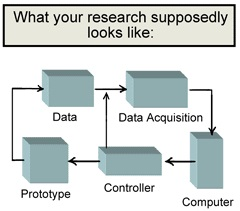
\includegraphics[width=8cm]{figuras/figura-1}}
		}{
			\Fonte{Elaborado pelo autor}
		}	
	\end{figure}
	
\lipsum[11]


\section{Fundamentação Teórica B}
\label{sec:fundamentacao-teorica-b}

Integer non lacinia magna. Aenean tempor lorem tellus, non sodales nisl commodo ut. Proin mattis placerat risus sit amet laoreet. Praesent sapien arcu, maximus ac fringilla efficitur, vulputate faucibus sem. Donec aliquet velit eros, sit amet elementum dolor pharetra eget. Integer eget mattis libero. Praesent ex velit, pulvinar at massa vel, fermentum dictum mauris. Ut feugiat accumsan augue, et ultrices ipsum euismod vitae

	\begin{figure}[h!]
		\centering
		\Caption{\label{fig:exemplo-2} Maecenas luctus augue odio, sed tincidunt nunc posuere nec}	
		\FBUNIfig{}{
			\fbox{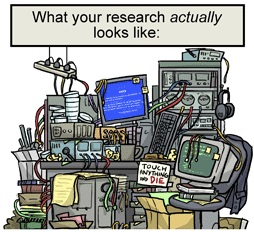
\includegraphics[width=8cm]{figuras/figura-2}}
		}{
			\Fonte{Elaborado pelo autor}			
		}	
	\end{figure}

Nunc ac pretium dui. Mauris aliquam dapibus nulla ac mattis. Aenean non tortor volutpat, varius lectus vitae, accumsan nibh. Cras pretium vestibulum enim, id ullamcorper tortor ultrices non. Integer sodales viverra faucibus. Curabitur at dui lacinia, rhoncus lacus at, blandit metus. Integer scelerisque non enim quis ornare.

\lipsum[13]

	\begin{table}[h!]	
		\centering
		\Caption{\label{tab:exemplo-1} Duis faucibus, enim quis tincidunt pellentesque, nisl leo varius nulla, vitae tempus dui mauris ac ante purus lorem}		
		\FBUNItab{}{
			\begin{tabular}{cll}
				\toprule
				Ranking & Exon Coverage & Splice Site Support \\
				\midrule \midrule
				E1 & Complete coverage by a single transcript & Both splice sites\\
				E2 & Complete coverage by more than a single transcript & Both splice sites\\
				E3 & Partial coverage & Both splice sites\\
				E4 & Partial coverage & One splice site\\
				E5 & Complete or partial coverage & No splice sites\\
				E6 & No coverage & No splice sites\\
				\bottomrule
			\end{tabular}
		}{
		\Fonte{Elaborado pelo autor}
	}
	\end{table}

Duis faucibus, enim quis tincidunt pellentesque, nisl leo varius nulla, vitae tempus dui mauris ac ante. Quisque purus lorem, pharetra sit amet lobortis eu, vehicula vitae purus. Ut varius, erat nec vehicula elementum, risus est tempus justo, nec vulputate augue leo egestas metus.

	\begin{figure}[h!]
		\centering
		\Caption{\label{fig:exemplo-3} Ut posuere, ex quis sagittis auctor, magna massa euismod felis}	
		\FBUNIfig{}{
			\fbox{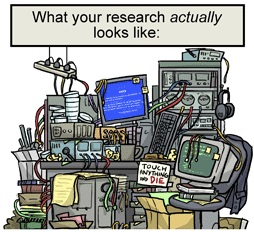
\includegraphics[width=8cm]{figuras/figura-2}}
		}{
		\Fonte{Elaborado pelo autor}			
	}	
	\end{figure}

\lipsum[14]

	\begin{table}[h!]	
		\centering
		\Caption{\label{tab:exemplo-2} Etiam molestie, nulla a egestas aliquet, velit augue congue metus}		
		\FBUNItab{}{
			\begin{tabular}{ccll}
				\toprule
				Quisque & pharetra & tempus & vulputate \\
				\midrule \midrule
				E1 & Complete coverage by a single transcript & Both splice sites\\
				E2 & Complete coverage by more than a single transcript & Both splice sites\\
				E3 & Partial coverage & Both splice sites & Both \\
				E4 & Partial coverage & One splice site & Both \\
				E5 & Complete or partial coverage & No splice sites & Both\\
				E6 & No coverage & No splice sites\\
				\bottomrule
			\end{tabular}
		}{
		\Fonte{Elaborado pelo autor}
	}
	\end{table}
	
Duis faucibus, enim quis tincidunt pellentesque, nisl leo varius nulla, vitae tempus dui mauris ac ante. Quisque purus lorem, pharetra sit amet lobortis eu, vehicula vitae purus.
%\acrlong{DATASUS},\acrlong{DNV},\acrlong{DO},\acrlong{ESF},\acrlong{IBGE},\acrlong{MFC},\acrlong{MI},\acrlong{MS},\acrlong{NV},\acrlong{ODM},\acrlong{OI},\acrlong{OMS},\acrlong{ONU},\acrlong{PNI},\acrlong{PSF},\acrlong{RIPSA},\acrlong{RN},\acrlong{SIM},\acrlong{SINASC},\acrlong{SUS},\acrlong{TMI},\acrlong{TMMFC}

\begin{alineascomponto}
	\item Integer non lacinia magna. Aenean tempor lorem tellus, non sodales nisl commodo ut
	\item Proin mattis placerat risus sit amet laoreet. Praesent sapien arcu, maximus ac fringilla efficitur, vulputate faucibus sem. Donec aliquet velit eros, sit amet elementum dolor pharetra eget
	\item Integer eget mattis libero. Praesent ex velit, pulvinar at massa vel, fermentum dictum mauris. Ut feugiat accumsan augue, et ultrices ipsum euismod vitae
	\begin{subalineascomponto}
		\item Integer non lacinia magna. Aenean tempor lorem tellus, non sodales nisl commodo ut
		\item Proin mattis placerat risus sit amet laoreet.
	\end{subalineascomponto}
\end{alineascomponto}
	\chapter{Trabalhos Relacionados}
\label{cap:trabalhos-relacionados}

Integer non lacinia magna. Aenean tempor lorem tellus, non sodales nisl commodo ut. Proin mattis placerat risus sit amet laoreet. Praesent sapien arcu, maximus ac fringilla efficitur, vulputate faucibus sem. Donec aliquet velit eros, sit amet elementum dolor pharetra eget. Integer eget mattis libero

\section{Trabalho Relacionado A}
\label{sec:trabalho-relacionado-a}

\lipsum[10]

	\begin{figure}[h!]
		\centering
		\Caption{\label{fig:exemplo-1} Lorem ipsum dolor sit amet, consectetur adipiscing elit. Suspendisse commodo lectus et augue elementum varius.}	
		\FBUNIfig{}{
			\fbox{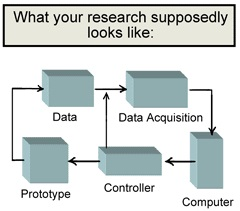
\includegraphics[width=8cm]{figuras/figura-1}}
		}{
			\Fonte{Elaborado pelo autor}
		}	
	\end{figure}
	
\lipsum[11]

\section{Trabalho Relacionado B}
\label{sec:trabalho-relacionado-b}

Integer non lacinia magna. Aenean tempor lorem tellus, non sodales nisl commodo ut. Proin mattis placerat risus sit amet laoreet. Praesent sapien arcu, maximus ac fringilla efficitur, vulputate faucibus sem. Donec aliquet velit eros, sit amet elementum dolor pharetra eget. Integer eget mattis libero. Praesent ex velit, pulvinar at massa vel, fermentum dictum mauris. Ut feugiat accumsan augue, et ultrices ipsum euismod vitae

	\begin{figure}[h!]
		\centering
		\Caption{\label{fig:exemplo-2} Maecenas luctus augue odio, sed tincidunt nunc posuere nec}	
		\FBUNIfig{}{
			\fbox{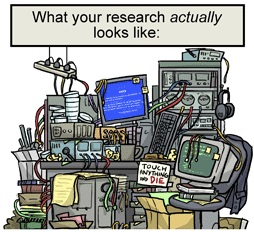
\includegraphics[width=8cm]{figuras/figura-2}}
		}{
			\Fonte{Elaborado pelo autor}			
		}	
	\end{figure}

Nunc ac pretium dui. Mauris aliquam dapibus nulla ac mattis. Aenean non tortor volutpat, varius lectus vitae, accumsan nibh. Cras pretium vestibulum enim, id ullamcorper tortor ultrices non. Integer sodales viverra faucibus. Curabitur at dui lacinia, rhoncus lacus at, blandit metus. Integer scelerisque non enim quis ornare.

	\begin{quadro}[h!]	
		\centering
		\Caption{\label{qua:exemplo-1} Praesent ex velit, pulvinar at massa vel, fermentum dictum mauris. Ut feugiat accumsan augue}		
		\FBUNIqua{}{
			\begin{tabular}{|c|c|l|l|}
				\hline
				Quisque & pharetra & tempus & vulputate \\
				\hline
				E1 & Complete coverage by a single transcript & Both  & Complete\\
				\hline
				E2 & Complete coverage by more than & Both splice sites & Complete\\
				\hline
				E3 & Partial coverage & Both splice sites & Both \\				
				\hline
			\end{tabular}
		}{
			\Fonte{Elaborado pelo autor}
		}
	\end{quadro}
	
\lipsum[20]

	
	\begin{quadro}[h!]	
		\centering
		\Caption{\label{qua:exemplo-2} Duis faucibus, enim quis tincidunt pellentesque}		
		\FBUNIqua{}{
			\begin{tabular}{|c|c|}
				\hline
				Quisque & pharetra \\
				\hline
				E1 & Complete coverage by a single transcript \\
				\hline
				E2 & Complete coverage by more than \\
				\hline
				E3 & Partial coverage \\
				\hline
				E4 & Partial coverage \\
				\hline
				E5 & Partial coverage \\
				\hline
				E6 & Partial coverage \\
				\hline
				E7 & Partial coverage \\
				\hline
			\end{tabular}
		}{
			\Fonte{Elaborado pelo autor}
		}
	\end{quadro}

\lipsum[21]

Integer non lacinia magna. Aenean tempor lorem tellus, non sodales nisl commodo ut. Proin mattis placerat risus sit amet laoreet. Praesent sapien arcu, maximus ac fringilla efficitur, vulputate faucibus sem. Donec aliquet velit eros, sit amet elementum dolor pharetra eget. Integer eget mattis libero.
\Gls{ambiguidade}
\Gls{braile}
\Gls{coerencia}
\Gls{dialetos}
\Gls{elipse}
\Gls{locucao-adjetiva}
\Gls{modificadores}
\Gls{paronimos}
\Gls{sintese}
\Gls{borboleta}
	\chapter{Metodologia}
\label{chap:metodologia}

\lipsum[2]
\lipsum[12]

O autor \cite{lamport1986latex} e \cite{Maia2011} \lipsum[2] 

\begin{table}[h!]
	\Caption{\label{tabela-ibge} Um Exemplo de tabela alinhada que pode ser longa ou curta, conforme padrão IBGE}%
	\IBGEtab{}{%
		\begin{tabular}{ccc}
			\toprule
			Nome & Nascimento & Documento \\
			\midrule \midrule
			Maria da Silva & 11/11/1111 & 111.111.111-11 \\
			Maria da Silva & 11/11/1111 & 111.111.111-11 \\
			Maria da Silva & 11/11/1111 & 111.111.111-11 \\
			\bottomrule
		\end{tabular}%
	}{%
	\Fonte{Produzido pelos autores}%
	\Nota{Esta é uma nota, que diz que os dados são baseados na
		regressão linear.}%
	\Nota[Anotações]{Uma anotação adicional, seguida de várias outras.}%
}
\end{table}

\cite{Huetal2000} \lipsum[2] 

\section{Exemplo de Algoritmos e Figuras}
\label{sec:exemplo-de-algoritmos-e-figuras}

\lipsum[2]

\begin{algorithm}[h!]
	\SetSpacedAlgorithm
	\caption{\label{exemplo-de-algoritmo}Como escrever algoritmos no \LaTeX2e}
	\Entrada{o proprio texto}
	\Saida{como escrever algoritmos com \LaTeX2e }
	\Inicio{
		inicializa\c{c}\~ao\;
		\Repita{fim do texto}{
			leia o atual\;
			\Se{entendeu}{
				vá para o próximo\;
				próximo se torna o atual\;}
			\Senao{volte ao início da seção\;}
		}
	}	
\end{algorithm}

\lipsum[2]
%\begin{algorithm}[H]
%	\Entrada{o proprio texto}
%	\Saida{como escrever algoritmos com \LaTeX2e }
%	\Inicio{
%		inicializa\c{c}\~ao\;
%		\Repita{fim do texto}{
%			leia o atual\;
%			\Se{entendeu}{
%				vá para o próximo\;
%				próximo se torna o atual\;}
%			\Senao{volte ao início da seção\;}
%		}
%	}
%	\caption{Exemplo de Algoritmo Versao 02}
%\end{algorithm}

%\begin{algorithm}
%	\begin{algorithmic}
%	\Entrada{o proprio texto}
%	\Saida{como escrever algoritmos com \LaTeX2e }	
%	\end{algorithmic}
%\end{algorithm}

Exemplo de alíneas com números:

\begin{alineascomnumero}
	\item Lorem ipsum dolor sit amet, consectetur adipiscing elit. Nunc dictum sed tortor nec viverra.
	\item Praesent vitae nulla varius, pulvinar quam at, dapibus nisi. Aenean in commodo tellus. Mauris molestie est sed justo malesuada, quis feugiat tellus venenatis.
	\item Praesent quis erat eleifend, lacinia turpis in, tristique tellus. Nunc dictum sed tortor nec viverra.
	\item Mauris facilisis odio eu ornare tempor. Nunc dictum sed tortor nec viverra.
	\item Curabitur convallis odio at eros consequat pretium.
\end{alineascomnumero}

\lipsum[12]

\begin{table}[h!]	
	\centering
	\Caption{\label{tab:internal}Internal exon scores}	
	\IBGEtab{}{
		\begin{tabular}{cll}
			\toprule
			Ranking & Exon Coverage & Splice Site Support\\
			\midrule \midrule
			E1 & Complete coverage by a single transcript & Both splice sites\\
			E2 & Complete coverage by more than a single transcript & Both splice sites\\
			E3 & Partial coverage & Both splice sites\\
			E4 & Partial coverage & One splice site\\
			E5 & Complete or partial coverage & No splice sites\\
			E6 & No coverage & No splice sites\\
			\bottomrule
		\end{tabular}
	}{
	\Fonte{os autores}
}
\end{table}

\lipsum[2] Referenciando a \autoref{tab:internal} \lipsum[2]

\index{figuras}Figuras podem ser criadas diretamente em LaTeX,
como o exemplo da \ref{fig-grafico-1}.

\begin{figure}[h!]
	\centering
	\Caption{\label{fig-grafico-1}Produção anual das dissertações de mestrado e teses de doutorado entre os anos de 1990 e 2008}		
	\IBGEtab{}{
		\fbox{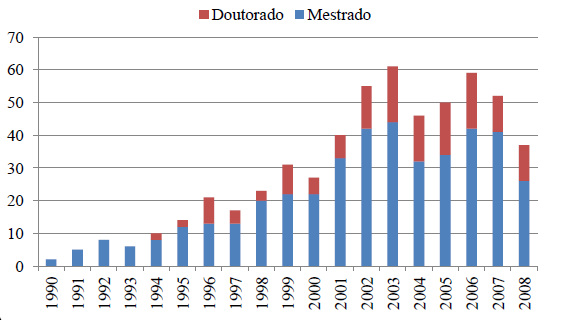
\includegraphics[scale=0.5]{figuras/figura-3}}
	}{
	\Fonte{os autores}
}
\end{figure}

Ou então figuras podem ser incorporadas de arquivos externos, como é o caso da \autoref{fig-grafico-1}. Se a figura que ser incluída se tratar de um diagrama, um gráfico ou uma ilustração que você mesmo produza, priorize o uso de imagens vetoriais no formato PDF. Com isso, o tamanho do arquivo final do trabalho será menor, e as imagens terão uma apresentação melhor, principalmente quando impressas, uma vez que imagens vetorias são perfeitamente escaláveis para qualquer dimensão. Nesse caso, se for utilizar o Microsoft Excel para produzir gráficos, ou o Microsoft Word para produzir ilustrações, exporte-os como PDF e os incorpore ao documento conforme o exemplo abaixo. No entanto, para manter a coerência no uso de software livre (já que você está usando LaTeX e abnTeX),  teste a ferramenta InkScape\index{InkScape}. ao CorelDraw\index{CorelDraw} ou ao Adobe Illustrator\index{Adobe! Illustrator}.  De todo modo, caso não seja possível  utilizar arquivos de imagens como PDF, utilize qualquer outro formato, como JPEG, GIF, BMP, etc.  Nesse caso, você pode tentar aprimorar as imagens incorporadas com o software livre \index{Gimp}Gimp. Ele é uma alternativa livre ao Adobe Photoshop\index{Adobe! Photoshop}.

\section{Usando Fórmulas Matemáticas}

\lipsum[2]

	\begin{equation}
		\begin{aligned}
			x = a_0 + \cfrac{1}{a_1
				+ \cfrac{1}{a_2
					+ \cfrac{1}{a_3 + \cfrac{1}{a_4} } } }
		\end{aligned}
	\end{equation}

\lipsum[3]

	\begin{equation}
		\begin{aligned}
			k_{n+1} = n^2 + k_n^2 - k_{n-1}
		\end{aligned}
	\end{equation}

\lipsum[4]

	\begin{equation}
		\begin{aligned}
			\cos (2\theta) = \cos^2 \theta - \sin^2 \theta
		\end{aligned}
	\end{equation}
	
\lipsum[5]

	\begin{equation}
		\begin{aligned}
			A_{m,n} =
			\begin{pmatrix}
			a_{1,1} & a_{1,2} & \cdots & a_{1,n} \\
			a_{2,1} & a_{2,2} & \cdots & a_{2,n} \\
			\vdots  & \vdots  & \ddots & \vdots  \\
			a_{m,1} & a_{m,2} & \cdots & a_{m,n}
			\end{pmatrix}
		\end{aligned}
	\end{equation}

\lipsum[6]

	\begin{equation}
		\begin{aligned}
			f(n) = \left\{ 
			\begin{array}{l l}
			n/2 & \quad \text{if $n$ is even}\\
			-(n+1)/2 & \quad \text{if $n$ is odd}
			\end{array} \right.
		\end{aligned}
	\end{equation}
	
\lipsum[7]

\section{Usando Algoritmos}

\lipsum[8]

\begin{algorithm}[h!]
	\SetSpacedAlgorithm
	\caption{\label{alg:algoritmo_de_colonica_de_formigas}Algoritmo de Otimização por Colônia de Formiga}
	\Entrada{Entrada do Algoritmo}
	\Saida{Saida do Algoritmo}
	\Inicio{
		Atribua os valores dos parâmetros\;
		Inicialize as trilhas de feromônios\;
		\Enqto{não atingir o critério de parada}{
			\Para{cada formiga}{
				Construa as Soluções\;
			}
			Aplique Busca Local (Opcional)\;
			Atualize o Feromônio\;
		}	
	}		
\end{algorithm}

\lipsum[9]

\section{Usando Código-fonte}

\lipsum[10]

\lstinputlisting[language=C++,caption={Hello World em C++}]{figuras/main.cpp}

\lipsum[11]

\begin{lstlisting}[language=Java,caption={Hello World em Java}]
public class HelloWorld {
	public static void main(String[] args) {
		System.out.println("Hello World!");
	}
}
\end{lstlisting}

\lipsum[11]

\section{Usando Teoremas, Proposições, etc}

Lorem ipsum dolor sit amet, consectetur adipiscing elit. Nunc dictum sed tortor nec viverra. consectetur adipiscing elit. Nunc dictum sed tortor nec viverra.

\begin{teo}[Pitágoras]
	Em todo triângulo retângulo o quadrado do comprimento da
	hipotenusa é igual a soma dos quadrados dos comprimentos dos catetos.
\end{teo}


Lorem ipsum dolor sit amet, consectetur adipiscing elit. Nunc dictum sed tortor nec viverra. consectetur adipiscing elit. Nunc dictum sed tortor nec viverra.

\begin{teo}[Fermat]
	Não existem inteiros $n > 2$, e $x, y, z$ tais que $x^n + y^n = z$
\end{teo}

Lorem ipsum dolor sit amet, consectetur adipiscing elit. Nunc dictum sed tortor nec viverra. consectetur adipiscing elit. Nunc dictum sed tortor nec viverra.

\begin{prop}
	Para demonstrar o Teorema de Pitágoras...
\end{prop}

Lorem ipsum dolor sit amet, consectetur adipiscing elit. Nunc dictum sed tortor nec viverra. consectetur adipiscing elit. Nunc dictum sed tortor nec viverra.

\begin{exem}
	Este é um exemplo do uso do ambiente exe definido acima.
\end{exem}

Lorem ipsum dolor sit amet, consectetur adipiscing elit. Nunc dictum sed tortor nec viverra. consectetur adipiscing elit. Nunc dictum sed tortor nec viverra.

\begin{xdefinicao}
	Definimos o produto de ...
\end{xdefinicao}

Lorem ipsum dolor sit amet, consectetur adipiscing elit. Nunc dictum sed tortor nec viverra. consectetur adipiscing elit. Nunc dictum sed tortor nec viverra.

\section{Usando Questões}


Lorem ipsum dolor sit amet, consectetur adipiscing elit. Nunc dictum sed tortor nec viverra. consectetur adipiscing elit. Nunc dictum sed tortor nec viverra.

\begin{questao}
	\item Esta é a primeira questão com alguns itens:
		\begin{enumerate}
			\item Este é o primeiro item
			\item Segundo item
		\end{enumerate}
	\item Esta é a segunda questão:
		\begin{enumerate}
			\item Este é o primeiro item
			\item Segundo item
		\end{enumerate}
	\item Lorem ipsum dolor sit amet, consectetur adipiscing elit. Nunc dictum sed tortor nec viverra. consectetur adipiscing elit. Nunc dictum sed tortor nec viverra.
		\begin{enumerate}
			\item consectetur
			\item adipiscing
			\item Nunc
			\item dictum
		\end{enumerate}
\end{questao}

\section{Citações}

\subsection{Documentos com três autores}

Quando houver três autores na citação, apresentam se os três, separados por ponto e vírgula, caso estes estejam após o texto. Se os autores estiverem incluídos no texto, devem ser separados por vírgula e pela conjunção "e".

\citeautoronline{tresautores}

\cite{tresautores}

\subsection{Documentos com mais de três autores}
Havendo mais de três autores, indica-se o primeiro seguido da expressão \textit{et al.} (do latim \textit{et alli}, que significa e outros), do ano e da página.

\citeautoronline{quatroautores}

\cite{quatroautores}

\subsection{Documentos de vários autores}

Havendo    citações    indiretas de    diversos    documentos    de    vários    autores, mencionados  simultaneamente e  que  expressam  a  mesma  ideia,  separam-se  os  autores  por ponto e vírgula, em ordem alfabética.

\cite{tresautores, quatroautores}

\section{Notas de Rodap\'{e}}

Deve-se utilizar o sistema autor-data para as  citações no texto e o numérico para notas explicativas\footnote{Veja - se como exemplo desse tipo de abordagem o estudo de Netzer (1976)}. As notas de rodapé podem e devem ser alinhadas, a partir da segunda linha da mesma nota, abaixo da primeira letra da primeira palavra, de forma a destacar o expoente \footnote{Encontramos  esse  tipo  de  perspectiva  na  2ª  parte  do  verbete  referido  na  nota  anterior,  em  grande  parte  do estudo de Rahner (1962).} e sem espaço entre elas e com fonte menor (tamanho 10).


	\chapter{Resultados}
\label{chap:resultados}

\lipsum[2]

\section{Resultados do Experimento A}
\label{sec:resultados-do-experimento-a}

\lipsum[3]

\section{Resultados do Experimento B}
\label{sec:resultados-do-experimento-b}

\lipsum[4]
	\chapter{Conclusões e Trabalhos Futuros}
\label{chap:conclusoes-e-trabalhos-futuros}

\lipsum[2]
\lipsum[34]

\section{Contribuições do Trabalho}
\label{sec:contribuicoes-do-trabalho}

\lipsum[3]

\section{Limitações}
\label{sec:limitacoes}

\lipsum[4]

\section{Trabalhos Futuros}
\label{sec:trabalhos-futuros}

\lipsum[5]






	%Elementos pós-textuais
	\bibliography{elementos-pos-textuais/referencias}
	\imprimirglossario
	\imprimirapendices
		% Adicione aqui os apendices do seu trabalho
		\apendice{Lorem Ipsum}
\label{ap:lorem-ipsum}

\lipsum[1]
		\apendice{Modelo de Capa}
\label{ap:modelo-de-capa}

\lipsum[1]

		\apendice{Termo de Fiel Depositário}
\label{ap:termo-de-fiel-depositario}

\noindent \textbf{Pesquisa:} ANÁLISE DA MORTALIDADE INFANTIL COM MALFORMAÇÕES CONGÊNITAS.

\noindent Pelo presente instrumento que atende às exigências legais, a Sra. Maria Consuelo Martins Saraiva, ``fiel depositário'' com o cargo de Secretária Municipal de Saúde de Iracema, após ter tomado conhecimento do protocolo de pesquisa intitulado: ANÁLISE DA MORTALIDADE INFANTIL COM MALFORMAÇÕES CONGÊNITAS. Analisando a repercussão desse estudo no contexto da saúde pública e epidemiologia, autoriza Karla Maria da Silva Lima, enfermeira, aluna do Curso de Mestrado Acadêmico em Enfermagem da Universidade Estadual do Ceará (UECE), sob orientação do Prof. Dr. José Maria de Castro, da UECE, ter acesso aos bancos de dados do Sistema de Informação sobre Nascidos Vivos e do Sistema de Informação sobre Mortalidade da Secretaria Municipal de Saúde de Iracema, objeto deste estudo, e que se encontram sob sua total responsabilidade. Fica claro que o Fiel Depositário pode a qualquer momento retirar sua AUTORIZAÇÃO e ciente de que todas as informações prestadas tornar-se-ão confidenciais e guardadas por força de sigilo profissional, assegurando que os dados obtidos da pesquisa serão somente utilizados para estudo.
	\imprimiranexos
		% Adicione aqui os anexos do seu trabalho
		\anexo{Exemplo de Anexo}
\label{an:exemplo-de-anexo}

\lipsum[13]
		\anexo{Dinâmica das classes sociais}
\label{an:dinamica-das-classes-sociais}

\lipsum[14]
\index{AAA}
	\imprimirindice

\end{document}
